\chapter{Evaluation of the \textit{i}MGXS Scheme}
\label{chap:results}

The preceding chapter introduced a methodology for \textit{inferential multi-group cross section} (\textit{i}\ac{MGXS}) spatial homogenization. The \textit{i}\ac{MGXS} scheme uses unsupervised clustering algorithms to infer the optimal assignment of fuel pin instances to spatial homogenization tally zones based on an analysis of ``noisy'' \ac{MC} tally data. This chapter evaluates the \textit{i}\ac{MGXS} homogenization with respect to the scheme's two primary objectives:

\begin{itemize}[noitemsep]
\item Approach the \textbf{accuracy} of \textit{degenerate} spatial homogenization (Sec.~\ref{subsec:chap8-degenerate})
\item Approach the \ac{MC} \textbf{convergence} of \textit{null} spatial homogenization (Sec.~\ref{subsec:chap8-null})
\end{itemize}

\noindent Furthermore, the \textit{i}\ac{MGXS} scheme seeks to address the shortcomings of the Local Neighbor Symmetry (\ac{LNS}) spatial homogenization scheme (Sec.~\ref{sec:chap9-lns-homogenize}) -- namely, its inability to flexibly distinguish \ac{MGXS} clusters in arbitrary geometries (\textit{e.g.}, pins along assembly-assembly and assembly-reflector interfaces) and its poor scalability for large geometries.

The results presented in this chapter reflect the key observations made in Chaps.~\ref{chap:quantify} and~\ref{chap:spatial} for the null, degenerate and \ac{LNS} homogenization schemes. First, it was observed that pin-wise homogenization with track density-weighted \ac{MGXS} (Sec.~\ref{subsec:chap8-fiss-rates}) has no impact on the resultant eigenvalue since all schemes preserve global reactivity. In addition, it was shown that pin-wise \ac{MGXS} clustering must be accounted for to accurately predict pin-wise U-238 capture rates, but it is much less consequential for accurate fission rate predictions. These results inform the results and analysis presented in this chapter.

The accuracy of the \textit{i}\ac{MGXS} scheme is evaluated with respect to the null and degenerate schemes in Sec.~\ref{subsec:chap11-imgxs-results}. The analysis includes a presentation of the eigenvalue bias and the distributions of pin-wise U-238 capture rate errors for four clustering algorithms (Sec.~\ref{sec:chap10-train-predictor}) with varying numbers of clusters, for each of the six heterogeneous \ac{PWR} benchmarks (Sec.~\ref{sec:chap7-benchmarks}). The convergence rate of the OpenMOC solutions with the null, degenerate and \textit{i}\ac{MGXS} schemes is presented in Sec.~\ref{sec:chap11-converge} for ``noisy'' \ac{MC} tally data computed with varying numbers of particle histories. Sec.~\ref{sec:chap11-model-select} examines the empirical results for model selection criteria (Sec.~\ref{sec:chap10-model-select}) which may be use to select the most appropriate number of clusters for the \textit{i}\ac{MGXS} scheme. Finally, Sec.~\ref{sec:chap11-synthesis} concludes with an analysis of the computational resource requirements for a reference \ac{MC} calculation in comparison to deterministic multi-group calculations with the degenerate and \textit{i}\ac{MGXS} schemes necessary to reach a desired level of accuracy for pin-wise U-238 capture rates.


%%%%%%%%%%%%%%%%%%%%%%%%%%%%%%%%%%%%%%%%%%%%%%%%%%%%%%%%%%%%%%%%%%%%%%%%%%%%%%%%
\section{Multi-Group Results with \textit{i}MGXS}
\label{subsec:chap11-imgxs-results}

Each of the six benchmarks was modeled with OpenMOC using \ac{MGXS} generated by the \textit{i}\ac{MGXS} spatial homogenization scheme. Each of the six heterogeneous benchmarks was modeled with 70-group \ac{MGXS} using the same OpenMOC runtime parameters as those used in Chap.~\ref{chap:quantify} for the infinite, null and degenerate homogenization, and in Chap.~\ref{chap:spatial} for \ac{LNS} homogenization. The eigenvalues and U-238 capture rates computed by OpenMOC are compared to the reference OpenMC solutions in Secs.~\ref{subsec:chap11-lns-eigenvalues} and~\ref{subsec:chap11-imgxs-capt-rates}, respectively.

-recall litmus-only feature selection - used in all cases!!!

second paragraph: OpenMC MGXS generation:
-100,000 particles / batch - individual assemblies
-100,000 particles / batch - 2x2 and reflector??
-1,000,000 particles / batch - quarter core
-10,000 batches for assemblies and reflector
-how many batches for full core??
-results may differ somewhat from those for null, degenerate and LNS schemes:
  -also used 1E9 total histories to evaluate other homogenization schemes
  -but those used 1E6 particles / batch, and thus only 8E8 active histories
  -these results are for 9.9E8 active histories since fewer particles per inactive batch

third paragraph: outline
-don't report on fission rates here
-Sec.~\ref{subsec:chap11-imgxs-eigenvalues}
-Sec.~\ref{subsec:chap11-imgxs-capt-rates}

%%%%%%%%%%%%%%%%%%%%%%%%
\subsection{Eigenvalues}
\label{subsec:chap11-imgxs-eigenvalues}

first paragraph: outline
-methodology:
  -recall litmus-only feature selection
  -recall four clustering algorithms
-eigenvalues should match those for null, degenerate and LNS schemes
  -don't expect clustering algorithm to have any impact on the eigenvaue bias
  -track density-weighted \ac{MGXS} preserves global reactivity

second paragraph: outline and analysis
-Tab.~\ref{table:chap11-eigenvalues}
  -benchmark
  -clustering algorithm
  -number of clusters
-remark on consistency for eigenvalues irregardless of number of clusters and clustering algorithm

The same trends highlighted in Sec.~\ref{subsec:chap8-eigenvalues} observed from the null and degenerate biases in Tab.~\ref{table:chap8-openmoc-eigenvalues} remain true for \ac{LNS} spatial homogenization. In fact, the \ac{LNS} eigenvalues are within 10 \ac{pcm} of those computed with both null and degenerate homogenization with 8 or more groups for all benchmarks. As previously noted in Sec.~\ref{subsec:chap8-eigenvalues}, this is expected since the \ac{MGXS} for the null, degenerate and \ac{LNS} schemes are homogenized from the same flux and should preserve globally-integrated reaction rates. Hence, \ac{LNS} homogenization is not expected to improve OpenMOC's eigenvalue predictions.

\begin{table}[ht!]
  \centering
  \caption[OpenMOC eigenvalue bias for litmus-only feature selection]{OpenMOC eigenvalue bias $\Delta\rho$ for \textit{i}\ac{MGXS} spatial homogenization with litmus-only feature selection.}
  \small
  \label{table:chap11-eigenvalues}
  \vspace{6pt}
  \begin{tabular}{l l R{1.2cm} R{1.2cm} R{1.2cm} R{1.2cm} R{1.2cm} R{1.2cm}}
  \toprule
  \rowcolor{lightgray}
  & \multicolumn{1}{c}{\cellcolor{lightgray} \bf Clustering} & \multicolumn{6}{S[table-format=6.1]}{\cellcolor{lightgray} \textbf{\# Clusters}} \\
  \multirow{-2}{*}{\cellcolor{lightgray} \bf Benchmark} &
  \multicolumn{1}{c}{\cellcolor{lightgray} \bf Algorithm} &
  \multicolumn{1}{c}{\cellcolor{lightgray} \bf 1\footnotemark} &
  \multicolumn{1}{c}{\cellcolor{lightgray} \bf 2} &
  \multicolumn{1}{c}{\cellcolor{lightgray} \bf 4} &
  \multicolumn{1}{c}{\cellcolor{lightgray} \bf 8} &
  \multicolumn{1}{c}{\cellcolor{lightgray} \bf 16} &
  \multicolumn{1}{c}{\cellcolor{lightgray} \bf \# pins\footnotemark} \\
  \midrule
\multirow{4}{*}{\parbox{2.5cm}{1.6\% Assm}} & Agglomerative & \multirow{4}{*}{-168} & -168 & -168 & -168 & -168 & \multirow{4}{*}{-168} \\
& BIRCH & & -168 & -168 & -168 & -168 & \\
& \ac{GMM} & & -168 & -168 & -168 & -168 & \\
& $k$-means & & -168 & -168 & -168 & -168 & \\
  \midrule
\multirow{4}{*}{\parbox{2.5cm}{3.1\% Assm}} & Agglomerative & \multirow{4}{*}{-194} & -194 & -194 & -194 & -194 & \multirow{4}{*}{-194} \\
& BIRCH & & -194 & -194 & -194 & -194 & \\
& \ac{GMM} & & -194 & -194 & -194 & -194 & \\
& $k$-means & & -194 & -194 & -194 & -194 & \\
  \midrule
\multirow{4}{*}{\parbox{2.5cm}{3.1\% Assm w/ 20 \acp{BP}}} & Agglomerative & \multirow{4}{*}{-240} & -237 & -236 & -235 & -235 & \multirow{4}{*}{-235} \\
& BIRCH & & -237 & -236 & -235 & -235 & \\
& \ac{GMM} & & -236 & -235 & -236 & -235 & \\
& $k$-means & & -236 & -236 & -236 & -235 & \\
  \midrule
\multirow{4}{*}{\parbox{2.5cm}{2$\times$2 Colorset}} & Agglomerative & \multirow{4}{*}{-191} & -189 & -189 & -189 & -189 & \multirow{4}{*}{-188} \\
& BIRCH & & -189 & -189 & -189 & -188 & \\
& \ac{GMM} & & -188 & -189 & -188 & -189 &  \\
& $k$-means & & -188 & -189 & -188 & -189 & \\
  \midrule
\multirow{4}{*}{\parbox{2.5cm}{2$\times$2 Colorset w/ Reflector}} & Agglomerative & \multirow{4}{*}{-141} & -136 & -136 & -134 & -129 & \multirow{4}{*}{-141} \\
& BIRCH & & -138 & -137 & -136 & -132 & \\
& \ac{GMM} & & -136 & -136 & -137 & -132 & \\
& $k$-means & & -136 & -136 & -134 & -132 & \\
  \midrule
\multirow{4}{*}{\parbox{2.5cm}{BEAVRS Full Core}} & Agglomerative & \multirow{4}{*}{-122} & -2125 & -120 & -119 & -119 & \multirow{4}{*}{-116} \\
& BIRCH & & -2541 & -120 & -120 & -119 & \\
& \ac{GMM} & & -2125 & -119 & -118 & -119 & \\
& $k$-means & & 4223 & -120 & -119 & -119 & \\
  \bottomrule
\end{tabular}
\end{table}

\addtocounter{footnote}{-2}
\stepcounter{footnote}
\footnotetext{\label{null}Null spatial homogenization is equivalent to \textit{i}\ac{MGXS} spatial homogenization with a single cluster.}

\stepcounter{footnote}
\footnotetext{\label{degenerate}Degenerate spatial homogenization is equivalent to \textit{i}\ac{MGXS} spatial homogenization with a unique cluster for each fuel pin instance.}

\clearpage

%%%%%%%%%%%%%%%%%%%%%%%%%%%%%%%%
\subsection{U-238 Capture Rates}
\label{subsec:chap11-imgxs-capt-rates}

first paragraph: outline
-methodology:
  -recall litmus-only feature selection - that is all that is used here
  -recall four clustering algorithms
-looking for two things:
  -1) want U-238 capture rates nearly as accurate as the degenerate case
        -perhaps even more accurate if MGXS are ``de-noised'', as was observed for LNS??
  -2) want to out-perform LNS for 2$\times$2 color with reflector and quarter core
  -3) want to compare different OpenMOC solutions to see relative impact of clustered \ac{MGXS}

second paragraph: outline
-Sec.~\ref{subsec:chap11-imgxs-capt-rates-num-clusters} - impact of number of clusters
-Sec.~\ref{subsec:chap11-imgxs-capt-rates-benchmark} - compare iMGXS with null and degenerate schemes
-Sec.~\ref{subsec:chap11-imgxs-capt-rates-space-distrib} - spatial distributions of U-238 capture errors
-Sec.~\ref{subsec:chap11-imgxs-capt-rates-compare} - compare OpenMOC solutions

%%%%%%%%%%%%%%%%%%%%%%%%%%%%%%%%%%%%%%%%%%%%%%%%%%%%%
\subsubsection{Variation with the Number of Clusters}
\label{subsec:chap11-imgxs-capt-rates-num-clusters}

first paragraph: objective
-quantify error with increasing number of clusters
-compare efficacy of the four clustering algorithms for the same number of clusters
-figures of capture rate percent relative errors by number of clusters
-Fig.~\ref{fig:chap11-coverge-complexity} - error with model complexity
  -expect diminishing returns with more clusters (greater model complexity)
  -expect the ``noisy'' in \ac{MC} tally data to minimize how close we can get to degenerate
  -a single cluster is equivalent to the null
  -a cluster for each pin is degenerate
  -will eventually approach the degenerate case with fully converged MGXS
    -dashed line for degenerate is with fully converged MGXS

second paragraph: outline and 
-Fig.~\Crefrange{fig:chap11-capt-err-by-cluster-assm-16}{fig:capt-err-by-cluster-assm-full-core} 
  -the max and mean errors for each of the benchmarks
    -individual assemblies, 2$\times$2 colorset and quarter core \ac{BEAVRS} model
-impact of clustering algorithm:
  -all algorithms within perform similarly for individual assemblies w/o \acp{BP}
  -KEY OBSERVATION:
    -with each successive addition of a cluster, best algorithm will discriminate those pins with the largest error into their own cluster
    -clustering algorithm does not have access to error
      -must make this distinction directly from \ac{MC} tally data
  -1) BIRCH seems to outperform other algorithms for 3.1\% assm with \acp{BP} and periodic colorset
    -achieving reduction from 0.7 -- 0.55\% in max rel. err. with only 6 clusters
      -GMM requires 8, agglomerative requires 9 and $k$-means requires 10      
    -dropoff may correspond to the discrimination of most limiting fuel pins into own cluster
    -distinction less clear for the reflected colorset
      -seems to require even more clusters (it does to reach degenerate's accuracy)
    -generally the most ``consistent'' and stable algorithm

third paragraph: impact of number of clusters:
-more clusters needed to reduce error for geometries with more complicated spatial heterogeneities
-in general, the mean is more limiting (requires more clusters) to converge/saturate
1) the majority of the reduction comes with the inclusion of just a few clusters
   -max err. for 1.6\% assm (1.1\%) eventually reduces to 0.45\%
   -just 3 clusters gets to 0.55\%, or 85\% of the reduction with just three clusters
2) more clusters needed as geometric complexities are added
   -add BPs
     -roughly 6 clusters needed for 3.1\% assm, while 10 or so needed with \acp{BP}
   -add reflector
     -perioridic colorset mean err saturated with 10 clusters
     -reflected colorset still trending downward even with 20 clusters

%-should mention errors with ICA, PCA, or FA to illustrate that clustering can screw up??? 
%-should mention errors look much different for pinch featur selection???

\begin{figure}[h!]
\centering
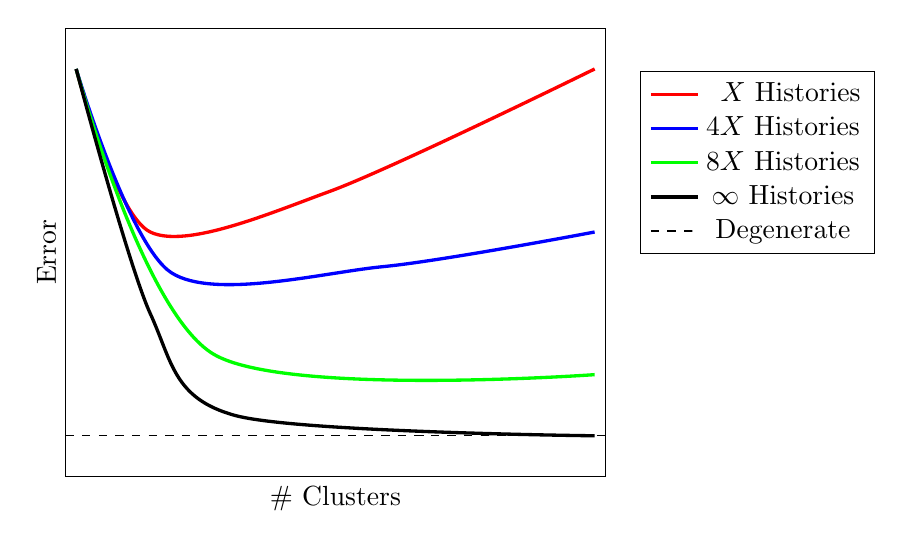
\begin{tikzpicture}
\begin{axis}[xmin=0,xmax=51,ymin=0,ymax=1.1,xlabel={\# Clusters},ylabel={Error},xticklabels={},yticklabels={},xtick={},ytick={},ticks=none,legend style={at={(1.5,0.7)},anchor=east,legend columns=1}]
\addplot[smooth,red,very thick] coordinates {
(1,1)
(8,0.6)
(25,0.7)
(50,1)
};
\addplot[smooth,blue,very thick] coordinates {
(1,1)
(10,0.5)
(30,0.515)
(50,0.6)
};
\addplot[smooth,green,very thick] coordinates {
(1,1)
(14,0.3)
(50,0.25)
};
\addplot[smooth,very thick] coordinates {
(1,1)
(8,0.4)
(16,0.15)
(50,0.1)
};
\addplot[smooth,dashed] coordinates {
(0,0.1)
(51,0.1)
};
\addlegendentry{$\;\;X$ Histories}
\addlegendentry{$4X$ Histories}
\addlegendentry{$8X$ Histories}
\addlegendentry{$\infty$ Histories}
\addlegendentry{Degenerate}
\end{axis}
\end{tikzpicture}
\caption[Convergence of\textit{i}MGXS to degenerate homogenization]{Convergence of \textit{i}\ac{MGXS} to degenerate homogenization in the limit of infinite particle histories.}
\label{fig:chap11-coverge-complexity}
\end{figure}

\begin{figure}[h!]
\centering
\begin{subfigure}{0.9\textwidth}
  \centering
  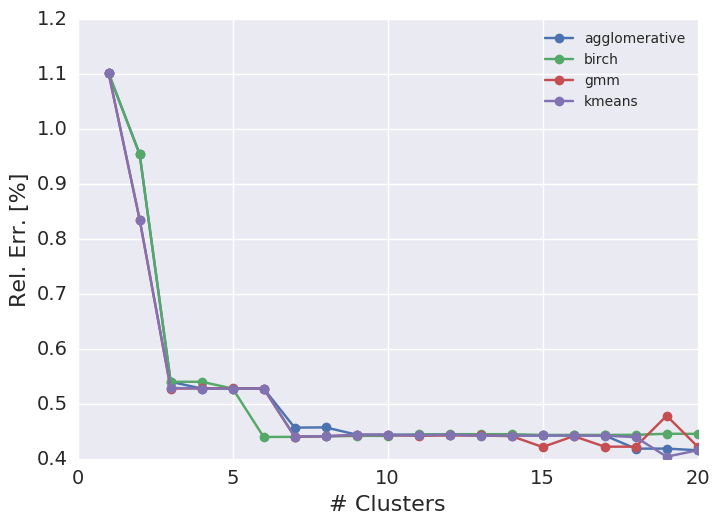
\includegraphics[width=\linewidth]{figures/results/err-by-cluster/assm-16/max-rel-err}
  \caption{}
  \label{fig:chap11-max-capt-err-by-cluster-assm-16}
\end{subfigure}
\begin{subfigure}{0.9\textwidth}
  \centering
  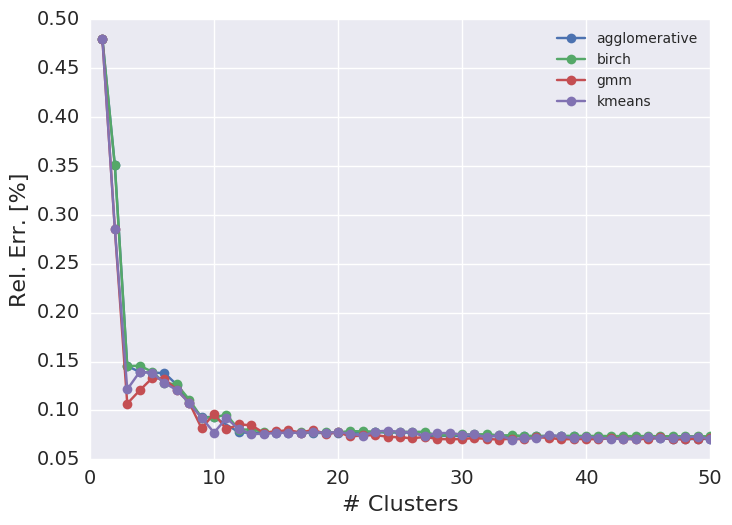
\includegraphics[width=\linewidth]{figures/results/err-by-cluster/assm-16/mean-rel-err}
  \caption{}
  \label{fig:chap11-mean-capt-err-by-cluster-assm-16}
\end{subfigure}
\caption[U-238 capture error for the 1.6\% enriched assembly]{The max (a) and mean (b) U-238 capture rate errors for the 1.6\% enriched assembly with \textit{i}\ac{MGXS} spatial homogenization.}
\label{fig:chap11-capt-err-by-cluster-assm-16}
\end{figure}

\begin{figure}[h!]
\centering
\begin{subfigure}{0.9\textwidth}
  \centering
  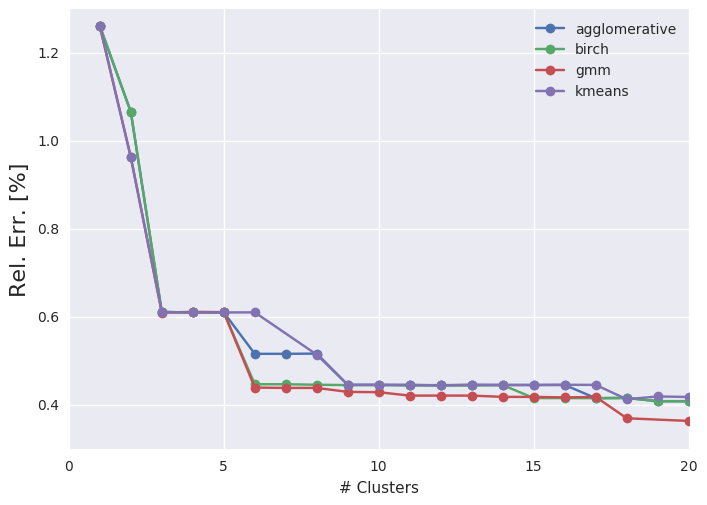
\includegraphics[width=\linewidth]{figures/results/err-by-cluster/assm-31/max-rel-err}
  \caption{}
  \label{fig:chap11-max-capt-err-by-cluster-assm-31}
\end{subfigure}
\begin{subfigure}{0.9\textwidth}
  \centering
  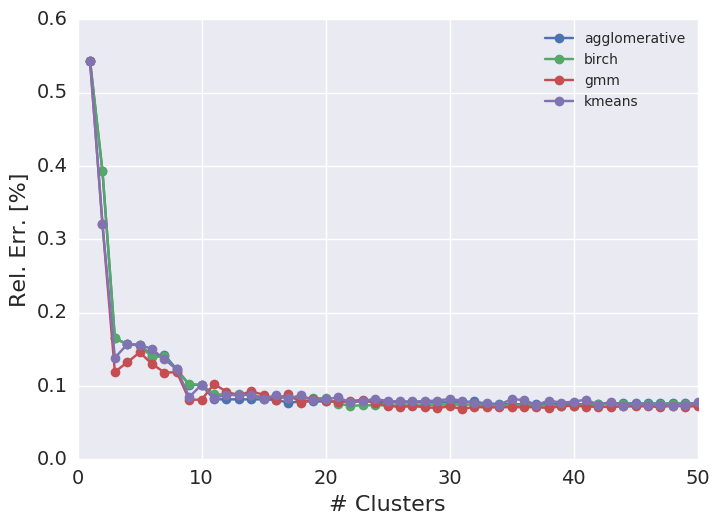
\includegraphics[width=\linewidth]{figures/results/err-by-cluster/assm-31/mean-rel-err}
  \caption{}
  \label{fig:chap11-mean-capt-err-by-cluster-assm-31}
\end{subfigure}
\caption[U-238 capture error for the 3.1\% enriched assembly]{The max (a) and mean (b) U-238 capture rate errors for the 3.1\% enriched assembly with \textit{i}\ac{MGXS} spatial homogenization.}
\label{fig:chap11-capt-err-by-cluster-assm-31}
\end{figure}

\begin{figure}[h!]
\centering
\begin{subfigure}{0.9\textwidth}
  \centering
  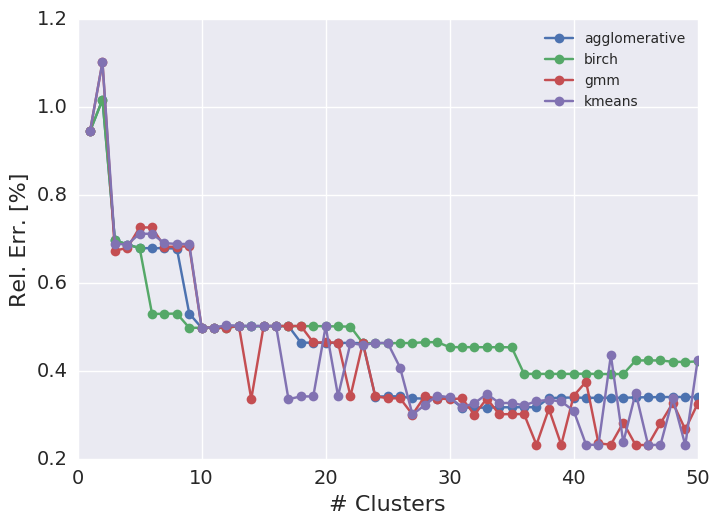
\includegraphics[width=\linewidth]{figures/results/err-by-cluster/assm-31-20BPs/max-rel-err}
  \caption{}
  \label{fig:chap11-max-capt-err-by-cluster-assm-31-20BPs}
\end{subfigure}
\begin{subfigure}{0.9\textwidth}
  \centering
  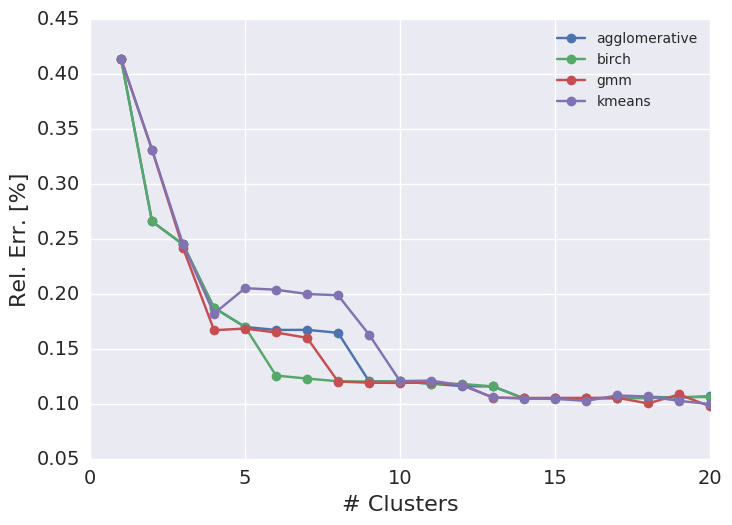
\includegraphics[width=\linewidth]{figures/results/err-by-cluster/assm-31-20BPs/mean-rel-err}
  \caption{}
  \label{fig:chap11-mean-capt-err-by-cluster-assm-31-20BPs}
\end{subfigure}
\caption[U-238 capture error the 3.1\% enriched assembly with 20 BPs]{The max (a) and mean (b) U-238 capture rate errors for the 3.1\% enriched assembly with 20 \acp{BP} with \textit{i}\ac{MGXS} spatial homogenization.}
\label{fig:chap11-capt-err-by-cluster-assm-31-20BPs}
\end{figure}

\begin{figure}[h!]
\centering
\begin{subfigure}{0.9\textwidth}
  \centering
  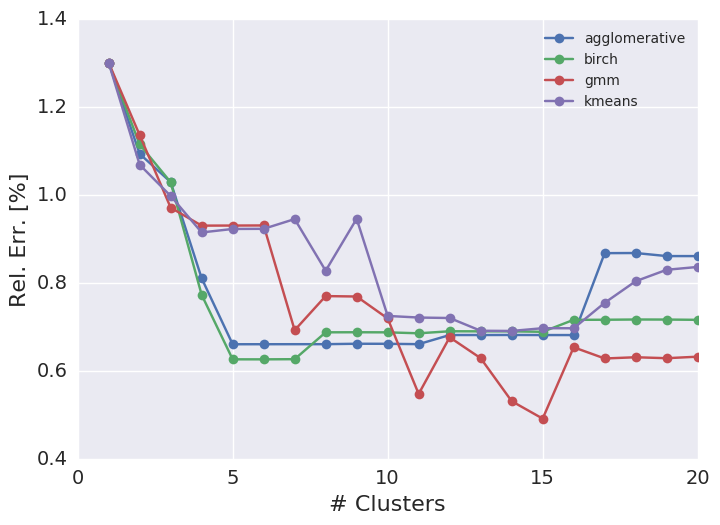
\includegraphics[width=\linewidth]{figures/results/err-by-cluster/2x2/max-rel-err}
  \caption{}
  \label{fig:chap11-max-capt-err-by-cluster-assm-2x2}
\end{subfigure}
\begin{subfigure}{0.9\textwidth}
  \centering
  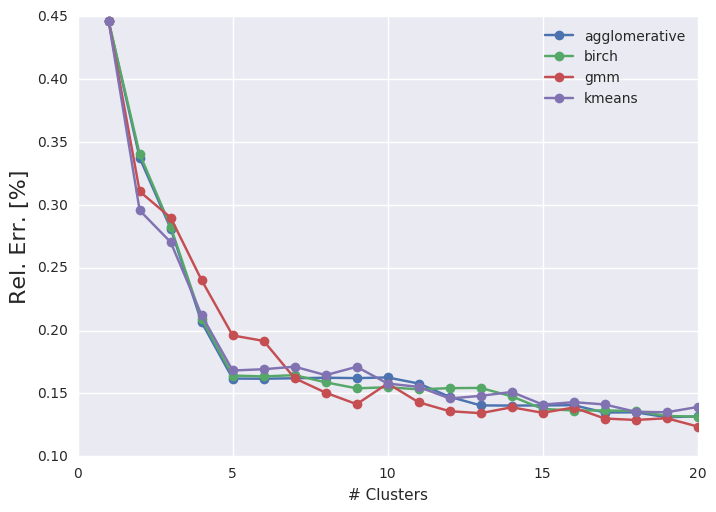
\includegraphics[width=\linewidth]{figures/results/err-by-cluster/2x2/mean-rel-err}
  \caption{}
  \label{fig:chap11-mean-capt-err-by-cluster-assm-2x2}
\end{subfigure}
\caption[U-238 capture error for the 2$\times$2 colorset]{The max (a) and mean (b) U-238 capture rate error for the 2$\times$2 colorset with \textit{i}\ac{MGXS} spatial homogenization.}
\label{fig:chap11-capt-err-by-cluster-assm-2x2}
\end{figure}

\begin{figure}[h!]
\centering
\begin{subfigure}{0.9\textwidth}
  \centering
  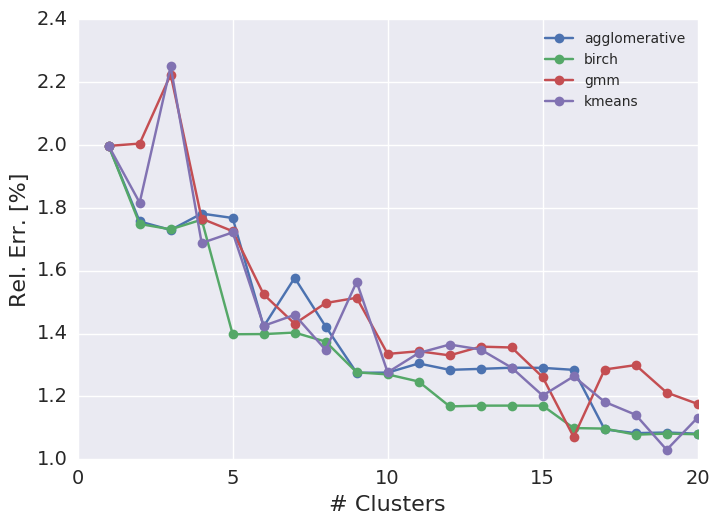
\includegraphics[width=\linewidth]{figures/results/err-by-cluster/reflector/max-rel-err}
  \caption{}
  \label{fig:chap11-max-capt-err-by-cluster-assm-refl}
\end{subfigure}
\begin{subfigure}{0.9\textwidth}
  \centering
  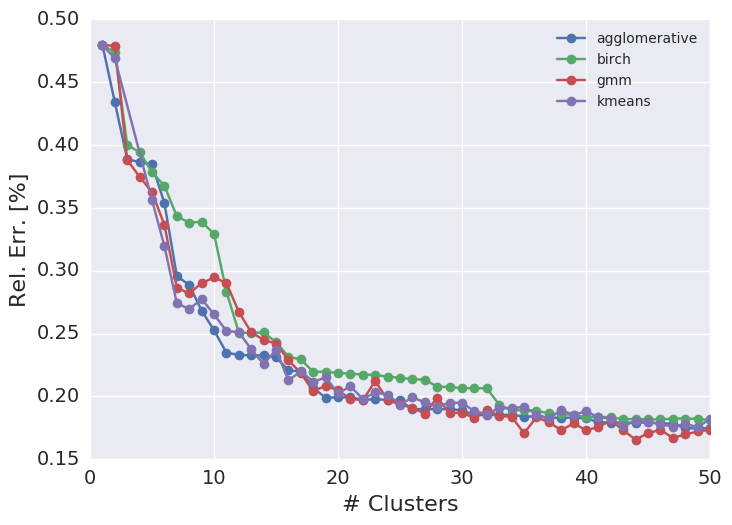
\includegraphics[width=\linewidth]{figures/results/err-by-cluster/reflector/mean-rel-err}
  \caption{}
  \label{fig:chap11-mean-capt-err-by-cluster-assm-refl}
\end{subfigure}
\caption[U-238 capture error for the 2$\times$2 colorset with reflector]{The max (a) and mean (b) U-238 capture rate error for the 2$\times$2 colorset with water reflector with \textit{i}\ac{MGXS} spatial homogenization.}
\label{fig:chap11-capt-err-by-cluster-assm-refl}
\end{figure}

\begin{figure}[h!]
\centering
\begin{subfigure}{0.9\textwidth}
  \centering
  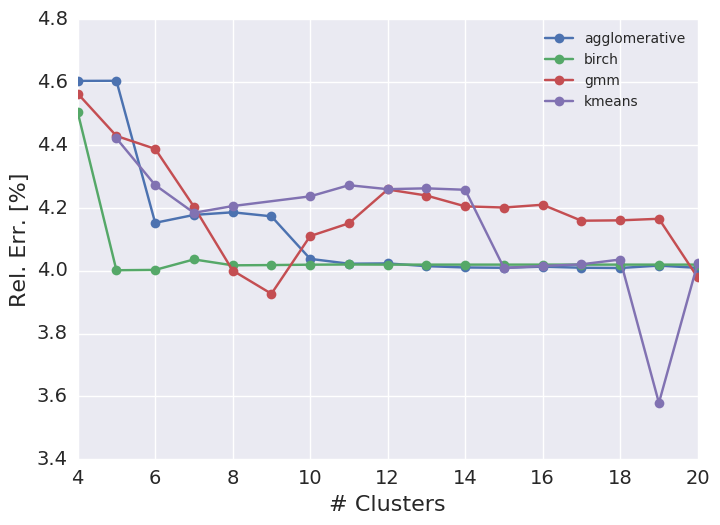
\includegraphics[width=\linewidth]{figures/results/err-by-cluster/full-core/max-rel-err}
  \caption{}
  \label{fig:max-capt-err-by-cluster-assm-full-core}
\end{subfigure}
\begin{subfigure}{0.9\textwidth}
  \centering
  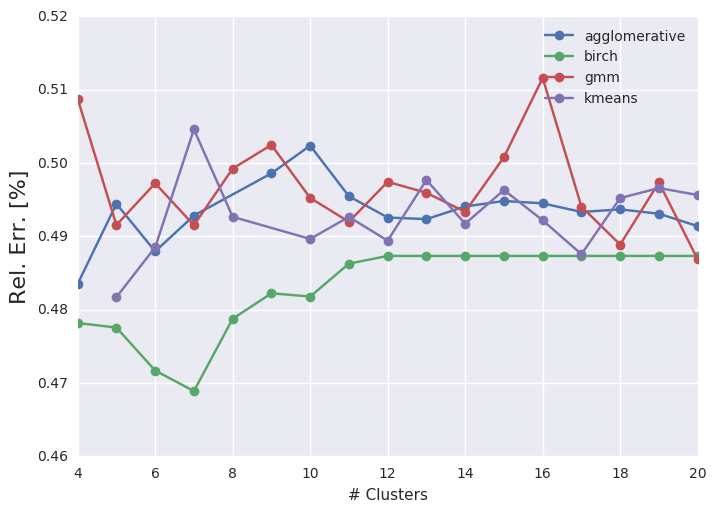
\includegraphics[width=\linewidth]{figures/results/err-by-cluster/full-core/mean-rel-err}
  \caption{}
  \label{fig:mean-capt-err-by-cluster-assm-full-core}
\end{subfigure}
\caption[U-238 capture error for quarter core BEAVRS model]{The max (a) and mean (b) U-238 capture rate error for the quarter core \ac{BEAVRS} model with \textit{i}\ac{MGXS} spatial homogenization.}
\label{fig:capt-err-by-cluster-assm-full-core}
\end{figure}

SUMMARY BOX

%%%%%%%%%%%%%%%%%%%%%%%%%%%%%%%%%%%%%%%%%%%%%%%%%%%%%%%%%%%%%%
\subsubsection{Benchmark with Null and Degenerate Schemes}
\label{subsec:chap11-imgxs-capt-rates-benchmark}

first paragraph: outline
-recall litmus-only feature selection
-Tabs.~\ref{table:chap11-max-capt-rates-litmus-only} and~\ref{table:chap11-mean-capt-rates-litmus-only}
-compare 1 (null) with 2 -- 16 clusters with the degenerate case

second paragraph: analysis
-by benchmark:
  -error increases 
-by algorithm:
  -largest differences are with the max err
    -BIRCH, GMM smaller errors (8 clusters) for 3.1\% assm w/ and w/o \acp{BP} 
    -BIRCH and GMM smaller errors (16 clusters) for reflected colorset
  -pretty consistent for mean err, recall discrepancies observed in preceding plots
-by number of clusters:
  -error always goes down, or stays relatively constant
  -16 clusters is enough to reduce the mean err to degenerate case for individual assms w/o \acp{BP}
    -not quite enough for the 3.1\% enriched assm with \acp{BP}
    -max err. is still quite a bit larger
  -in all cases (save for the periodic colorset)

The OpenMOC energy-integrated pin-wise U-238 capture rates were compared to the reference OpenMC fission rates for \ac{LNS} homogenization. The percent relative errors for each pin's fission rates were computed and the maximum and mean errors are listed for each benchmark and energy group structure in Tab.~\ref{table:chap9-lns-capture-rates}, respectively. In particular, the maximum errors are the maximum of the absolute values of the errors along with the appropriate sign, while the mean errors are the averages of the absolute error magnitudes. The results in Tab.~\ref{table:chap9-lns-capture-rates} can be compared to the corresponding data for infinite, null and degenerate homogenization in Tabs.~\ref{table:chap8-openmoc-max-capt-rates} and~\ref{table:chap8-openmoc-mean-capt-rates}. The 70-group degenerate results are reproduced in Tab.~\ref{table:chap9-lns-capture-rates} to simplify comparison with \ac{LNS}.

\begin{table}[h!]
  \centering
  \caption[Maximum OpenMOC U-238 capture rate errors]{Maximum absolute U-238 capture rate percent relative errors for \textit{i}\ac{MGXS} spatial homogenization.}
  \small
  \label{table:chap11-max-capt-rates}
  \vspace{6pt}
  \begin{tabular}{l l R{1.2cm} R{1.2cm} R{1.2cm} R{1.2cm} R{1.2cm} R{1.2cm}}
  \toprule
  \rowcolor{lightgray}
  & \multicolumn{1}{c}{\cellcolor{lightgray} \bf Clustering} & \multicolumn{6}{S[table-format=6.1]}{\cellcolor{lightgray} \textbf{\# Clusters}} \\
  \multirow{-2}{*}{\cellcolor{lightgray} \bf Benchmark} &
  \multicolumn{1}{c}{\cellcolor{lightgray} \bf Algorithm} &
  \multicolumn{1}{c}{\cellcolor{lightgray} \bf 1\textsuperscript{\ref{null}}} &
  \multicolumn{1}{c}{\cellcolor{lightgray} \bf 2} &
  \multicolumn{1}{c}{\cellcolor{lightgray} \bf 4} &
  \multicolumn{1}{c}{\cellcolor{lightgray} \bf 8} &
  \multicolumn{1}{c}{\cellcolor{lightgray} \bf 16} &
  \multicolumn{1}{c}{\cellcolor{lightgray} \bf \# pins\textsuperscript{\ref{degenerate}}} \\
  \midrule
\multirow{4}{*}{\parbox{2.5cm}{1.6\% Assm}} & Agglomerative & \multirow{4}{*}{-1.10} & 0.95 & -0.53 & -0.46 & -0.44 & \multirow{4}{*}{0.38} \\
& BIRCH & & 0.95 & -0.54 & -0.44 & -0.44 & \\
& \ac{GMM} & & -0.84 & -0.53 & -0.44 & -0.44 & \\
& $k$-means & & -0.84 & -0.53 & -0.44 & -0.44 & \\
  \midrule
\multirow{4}{*}{\parbox{2.5cm}{3.1\% Assm}} & Agglomerative & \multirow{4}{*}{-1.26} & 1.07 & -0.61 & -0.52 & 0.45 & \multirow{4}{*}{-0.33} \\
& BIRCH & & 1.07 & -0.61 & 0.45 & -0.42 & \\
& \ac{GMM} & & -0.96 & -0.61 & -0.44 & -0.42 & \\
& $k$-means & & -0.96 & -0.61 & -0.52 & 0.45 & \\
  \midrule
\multirow{4}{*}{\parbox{2.5cm}{3.1\% Assm w/ 20 BPs}} & Agglomerative & \multirow{4}{*}{-0.95} & -1.02 & 0.69 & 0.68 & -0.50 & \multirow{4}{*}{-0.30} \\
& BIRCH & & -1.02 & 0.69 & -0.53 & -0.50 & \\
& \ac{GMM} & & -1.10 & 0.68 & -0.53 & -0.50 & \\
& $k$-means & & -1.10 & 0.69 & -0.69 & 0.34 & \\
  \midrule
\multirow{4}{*}{\parbox{2.5cm}{2$\times$2 Colorset}} & Agglomerative & \multirow{4}{*}{-1.30} & -1.09 & 0.81 & 0.66 & 0.68 & \multirow{4}{*}{-0.64} \\
& BIRCH & & -1.12 & 0.77 & 0.69 & 0.72 & \\
& \ac{GMM} & & -1.14 & 0.93 & 0.77 & 0.65 & \\
& $k$-means & & -1.07 & -0.92 & -0.83 & 0.70 & \\
  \midrule
\multirow{4}{*}{\parbox{2.5cm}{2$\times$2 Colorset w/ Reflector}} & Agglomerative & \multirow{4}{*}{-2.00} & -1.76 & -1.78 & -1.42 & -1.28 & \multirow{4}{*}{-0.80} \\
& BIRCH & & -1.75 & -1.76 & -1.37 & 1.10 & \\
& \ac{GMM} & & -2.00 & -1.77 & 1.50 & 1.07 & \\
& $k$-means & & -1.82 & -1.69 & 1.35 & -1.26 & \\
  \midrule
\multirow{4}{*}{\parbox{2.5cm}{BEAVRS Full Core}} & Agglomerative & \multirow{4}{*}{-4.78} & 329.46 & -4.60 & -4.19 & -4.01 & \multirow{4}{*}{-3.03} \\
& BIRCH & & 851.56 & -4.51 & -4.02 & -4.02 & \\
& \ac{GMM} & & 329.46 & -4.56 & -4.00 & -4.21 & \\
& $k$-means & & 97.56 & -4.61 & -4.21 & -4.02 & \\
  \bottomrule
\end{tabular}
\end{table}

\clearpage

\begin{table}[h!]
  \centering
  \caption[Mean OpenMOC U-238 capture rate errors]{Mean absolute U-238 capture rate percent relative errors for \textit{i}\ac{MGXS}.}
  \small
  \label{table:chap11-mean-capt-rates}
  \vspace{6pt}
  \begin{tabular}{l l R{1.2cm} R{1.2cm} R{1.2cm} R{1.2cm} R{1.2cm} R{1.2cm}}
  \toprule
  \rowcolor{lightgray}
  & \multicolumn{1}{c}{\cellcolor{lightgray} \bf Clustering} & \multicolumn{6}{S[table-format=6.1]}{\cellcolor{lightgray} \textbf{\# Clusters}} \\
  \multirow{-2}{*}{\cellcolor{lightgray} \bf Benchmark} &
  \multicolumn{1}{c}{\cellcolor{lightgray} \bf Algorithm} &
  \multicolumn{1}{c}{\cellcolor{lightgray} \bf 1\textsuperscript{\ref{null}}} &
  \multicolumn{1}{c}{\cellcolor{lightgray} \bf 2} &
  \multicolumn{1}{c}{\cellcolor{lightgray} \bf 4} &
  \multicolumn{1}{c}{\cellcolor{lightgray} \bf 8} &
  \multicolumn{1}{c}{\cellcolor{lightgray} \bf 16} &
  \multicolumn{1}{c}{\cellcolor{lightgray} \bf \# pins\textsuperscript{\ref{degenerate}}} \\
  \midrule
\multirow{4}{*}{\parbox{2.5cm}{1.6\% Assm}} & Agglomerative & \multirow{4}{*}{0.48} & 0.35 & 0.14 & 0.11 & 0.08 & \multirow{4}{*}{0.08} \\
& BIRCH & & 0.35 & 0.15 & 0.11 & 0.08 & \\
& \ac{GMM} & & 0.29 & 0.12 & 0.11 & 0.08 & \\
& $k$-means & & 0.29 & 0.14 & 0.11 & 0.08 & \\
  \midrule
\multirow{4}{*}{\parbox{2.5cm}{3.1\% Assm}} & Agglomerative & \multirow{4}{*}{0.54} & 0.39 & 0.16 & 0.12 & 0.08 & \multirow{4}{*}{0.09} \\
& BIRCH & & 0.39 & 0.16 & 0.12 & 0.08 \\
& \ac{GMM} & & 0.32 & 0.13 & 0.10 & 0.09 & \\
& $k$-means & & 0.32 & 0.16 & 0.12 & 0.09 & \\
  \midrule
\multirow{4}{*}{\parbox{2.5cm}{3.1\% Assm w/ 20 BPs}} & Agglomerative & \multirow{4}{*}{0.41} & 0.27 & 0.19 & 0.17 & 0.11 & \multirow{4}{*}{0.09} \\
& BIRCH & & 0.27 & 0.19 & 0.12 & 0.11 & \\
& \ac{GMM} & & 0.33 & 0.17 & 0.12 & 0.11 & \\
& $k$-means & & 0.33 & 0.18 & 0.20 & 0.10 & \\
  \midrule
\multirow{4}{*}{\parbox{2.5cm}{2$\times$2 Colorset}} & Agglomerative & \multirow{4}{*}{0.45} & 0.34 & 0.21 & 0.16 & 0.14 & \multirow{4}{*}{0.15} \\
& BIRCH & & 0.34 & 0.21 & 0.16 & 0.14 & \\
& \ac{GMM} & & 0.31 & 0.24 & 0.15 & 0.14 & \\
& $k$-means & & 0.30 & 0.21 & 0.16 & 0.14 & \\
  \midrule
\multirow{4}{*}{\parbox{2.5cm}{2$\times$2 Colorset w/ Reflector}} & Agglomerative & \multirow{4}{*}{0.48} & 0.43 & 0.39 & 0.29 & 0.22 & \multirow{4}{*}{0.16} \\
& BIRCH & & 0.47 & 0.39 & 0.34 & 0.23 & \\
& \ac{GMM} & & 0.48 & 0.37 & 0.29 & 0.24 & \\
& $k$-means & & 0.47 & 0.37 & 0.27 & 0.22 & \\
  \midrule
\multirow{4}{*}{\parbox{2.5cm}{BEAVRS Full Core}} & Agglomerative & \multirow{4}{*}{0.49} & 83.89 & 0.48 & 0.49 & 0.49 & \multirow{4}{*}{0.39} \\
& BIRCH & & 128.76 & 0.48 & 0.48 & 0.49 & \\
& \ac{GMM} & & 83.89 & 0.51 & 0.50 & 0.51 & \\
& $k$-means & & 38.49 & 0.50 & 0.49 & 0.49 & \\
  \bottomrule
\end{tabular}
\end{table}

\clearpage

%%%%%%%%%%%%%%%%%%%%%%%%%%%%%%%%%%%%%%%%%%%%%%%%%%%%%%%%%%%%%%%%%%
\subsubsection{Spatial Distributions of U-238 Capture Rate Errors}
\label{subsec:chap11-imgxs-capt-rates-space-distrib}

first paragraph: outline
-Fig.~\Crefrange{fig:chap11-assm-1.6-capt-err}{fig:chap11-reflector-capt-err}
  -individual assemblies and colorsets
-Fig.~\Crefrange{fig:chap11-full-core-capt-err-a}{fig:chap11-full-core-capt-err-b}
  -full core
-compare errors with null, degenerate and \ac{LNS} spatial homogenization
-use the BIRCH clustering scheme for \textit{i}\ac{MGXS} with 2, 4 and 16 clusters

second paragraph: analysis
-need more clusters than \ac{LNS} for individual assemblies and periodic colorset
-even with 16 clusters do not quite approach degenerate's accuracy
-note that \ac{LNS} did better than degenerate for each benchmark except for reflected colorset
-periodic colorset:
  -even with 16 clusters, pins adjacent to two \acp{CRGT} (facial and diagonal) are not discriminated
  -\ac{LNS} discriminates these pins
  -\textit{i}\ac{MGXS} is expending clusters to discriminate pins along different assembly interfaces instead of discriminating the pins near \acp{CRGT}
    -this behavior is wholly dependent on the features used
-reflected colorset:
  -Fig.~\ref{fig:chap11-reflector-capt-err}
  -\textit{i}\ac{MGXS} does a better job along the assembly-reflector interface
-some lingering residual errors along assembly-assembly interfaces for reflected colorset
  -less so than \ac{LNS}

\begin{figure}[h!]
\centering
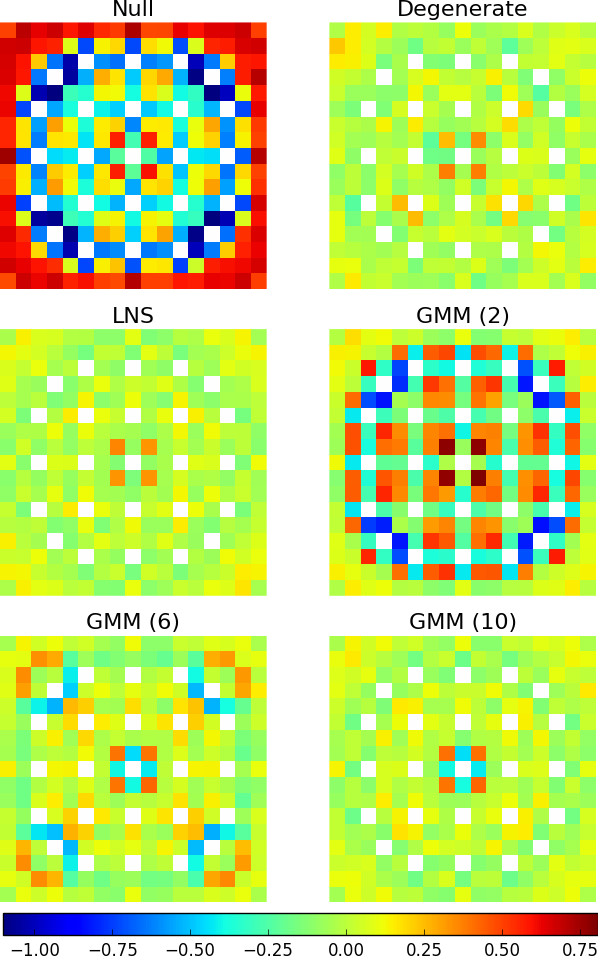
\includegraphics[width=0.9\linewidth]{figures/results/spatial/assm-16/capt-err}
\vspace{2mm}
\caption[U-238 capture errors for the 1.6\% enriched assembly]{U-238 capture percent relative errors for the 1.6\% enriched assembly with null, degenerate, \ac{LNS} and \textit{i}\ac{MGXS} spatial homogenization.}
\label{fig:chap11-assm-1.6-capt-err}
\end{figure}

\clearpage

\begin{figure}[h!]
\centering
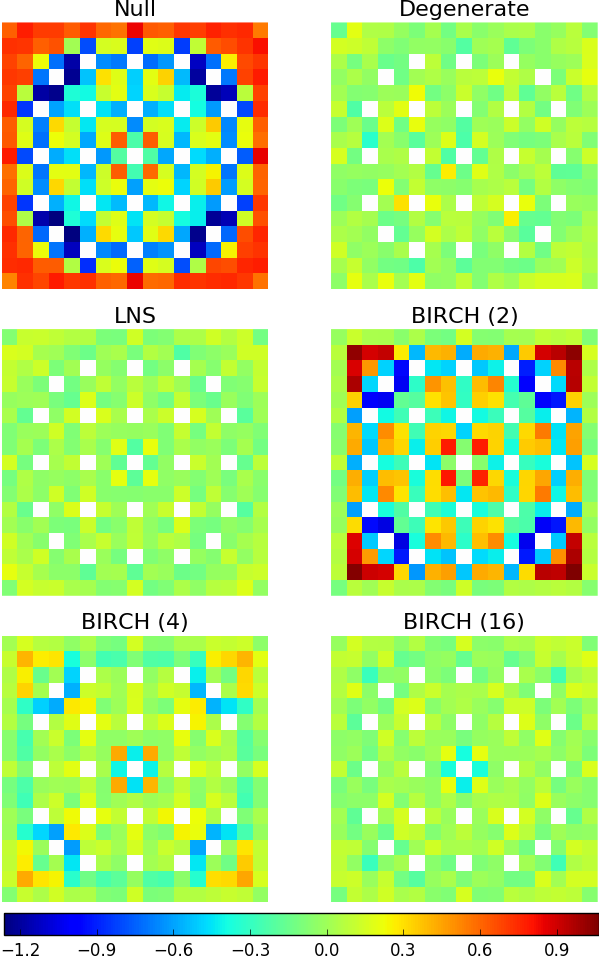
\includegraphics[width=0.9\linewidth]{figures/results/spatial/assm-31/capt-err}
\vspace{2mm}
\caption[U-238 capture errors for the 3.1\% enriched assembly]{U-238 capture percent relative errors for the 3.1\% enriched assembly with null, degenerate, \ac{LNS} and \textit{i}\ac{MGXS} spatial homogenization.}
\label{fig:chap11-assm-3.1-capt-err}
\end{figure}

\clearpage

\begin{figure}[h!]
\centering
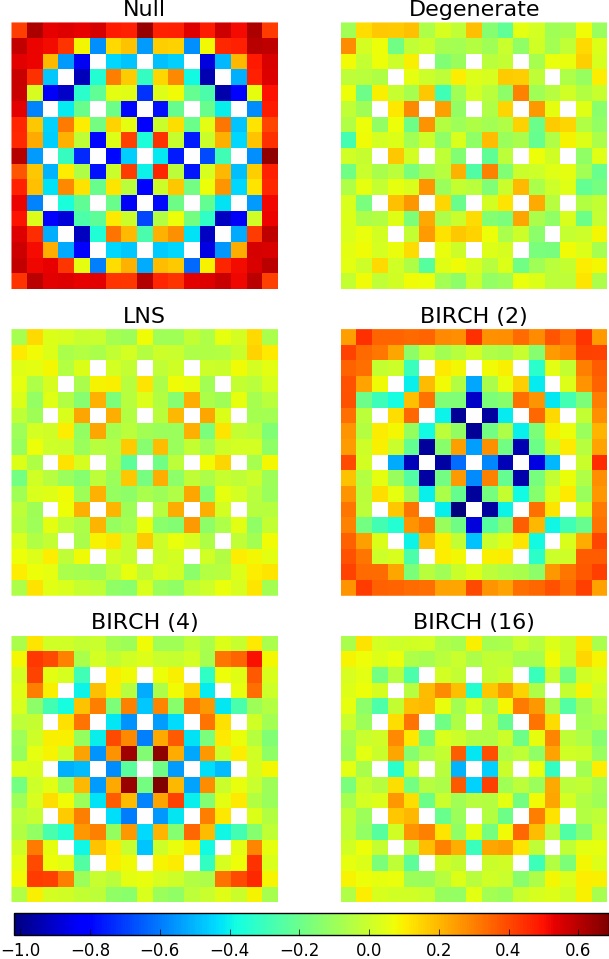
\includegraphics[width=0.9\linewidth]{figures/results/spatial/assm-31-20BPs/capt-err}
\vspace{2mm}
\caption[U-238 capture errors for the 3.1\% enriched assembly with 20 BPs]{U-238 capture percent relative errors for the 3.1\% enriched assembly with 20 \acp{BP} with null, degenerate, \ac{LNS} and \textit{i}\ac{MGXS} spatial homogenization.}
\label{fig:chap11-assm-3.1-20BPs-capt-err}
\end{figure}

\clearpage

\begin{figure}[h!]
\centering
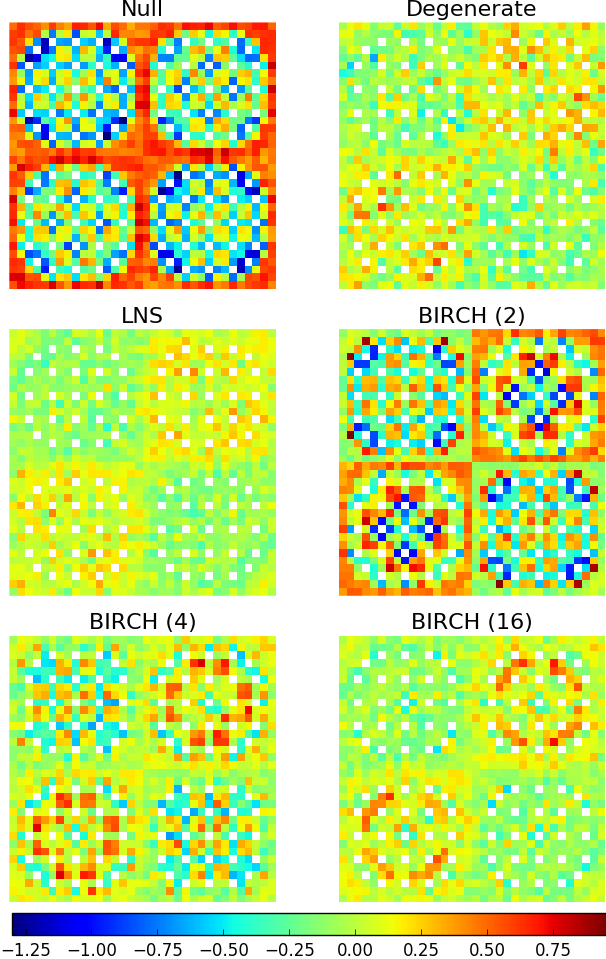
\includegraphics[width=0.9\linewidth]{figures/results/spatial/2x2/capt-err}
\vspace{2mm}
\caption[U-238 capture errors for the 2$\times$2 colorset]{U-238 capture percent relative errors for the 2$\times$2 colorset with null, degenerate, \ac{LNS} and \textit{i}\ac{MGXS} spatial homogenization.}
\label{fig:chap11-2x2-capt-err}
\end{figure}

\clearpage

\begin{figure}[h!]
\centering
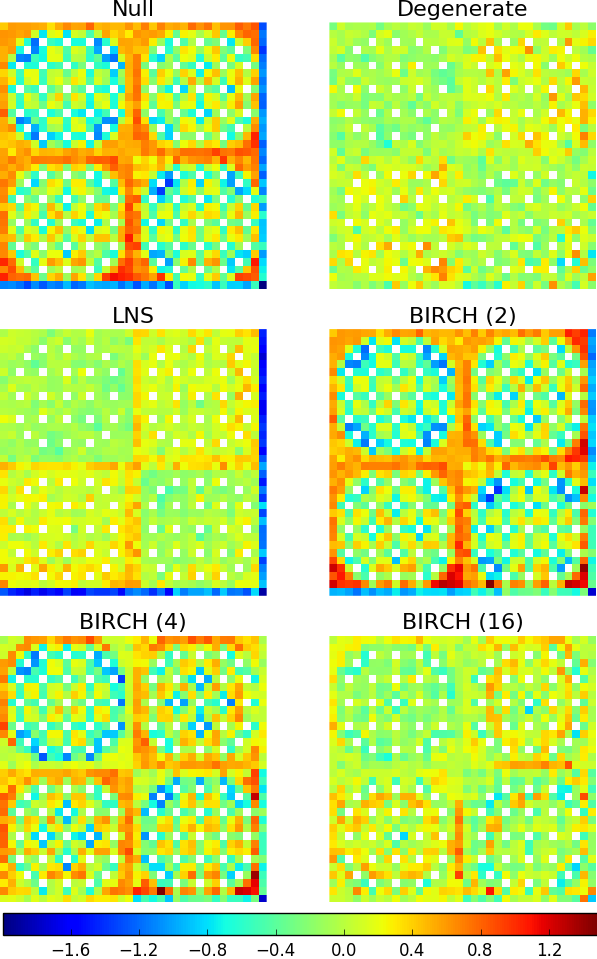
\includegraphics[width=0.9\linewidth]{figures/results/spatial/reflector/capt-err}
\vspace{2mm}
\caption[U-238 capture errors for the 2$\times$2 colorset with reflector]{U-238 capture percent relative errors for the 2$\times$2 colorset with a water reflector with null, degenerate, \ac{LNS} and \textit{i}\ac{MGXS} spatial homogenization.}
\label{fig:chap11-refl-capt-err}
\end{figure}

\clearpage

\begin{figure}[h!]
\centering
\begin{subfigure}{0.9\textwidth}
  \centering
  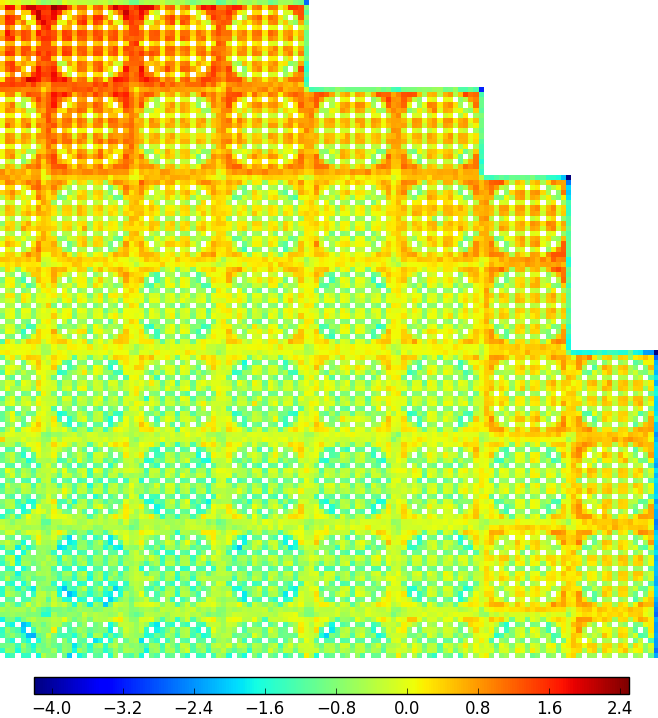
\includegraphics[width=0.65\linewidth]{figures/results/spatial/full-core/capt-err-null}
  \caption{}
  \label{fig:chap11-full-core-capt-err-null}
\end{subfigure}
\begin{subfigure}{0.9\textwidth}
  \centering
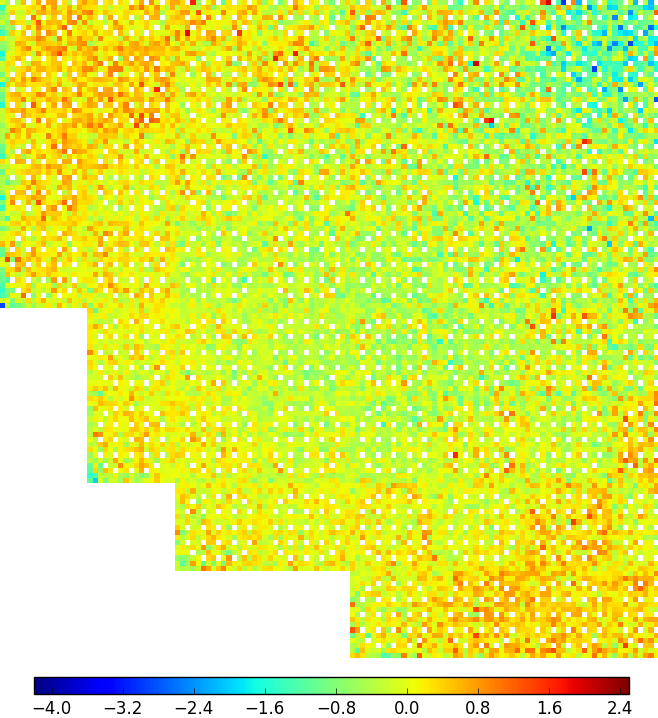
\includegraphics[width=0.65\linewidth]{figures/results/spatial/full-core/capt-err-degenerate}
  \caption{}
  \label{fig:chap11-full-core-capt-err-degenerate}
\end{subfigure}
\caption[U-238 capture rate errors for \ac{BEAVRS}]{U-238 capture percent relative errors for the quarter core \ac{BEAVRS} model with null (a) and degenerate (b) spatial homogenization.}
\label{fig:chap11-full-core-capt-err-a}
\end{figure}

\clearpage

\begin{figure}[h!]
\centering
\begin{subfigure}{0.9\textwidth}
  \centering
  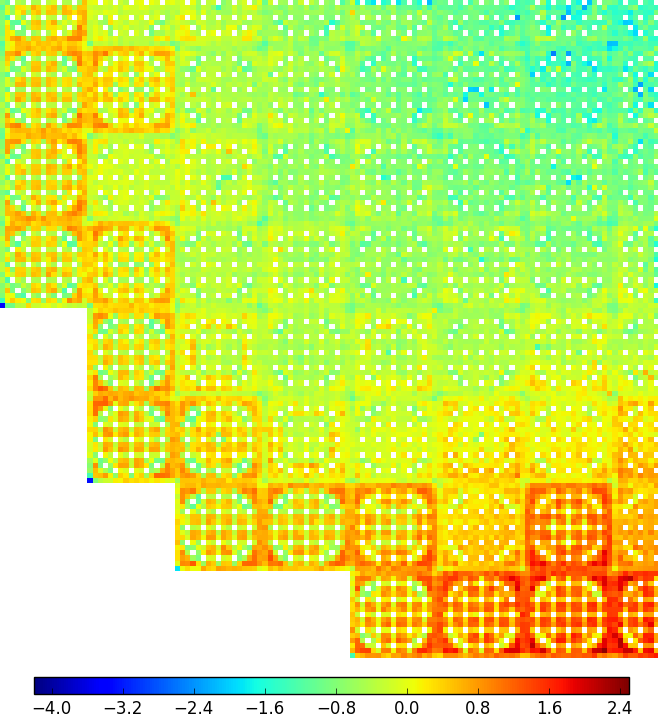
\includegraphics[width=0.65\linewidth]{figures/results/spatial/full-core/capt-err-birch-4}
  \caption{}
  \label{fig:chap11-full-core-capt-err-birch-4}
\end{subfigure}
\begin{subfigure}{0.9\textwidth}
  \centering
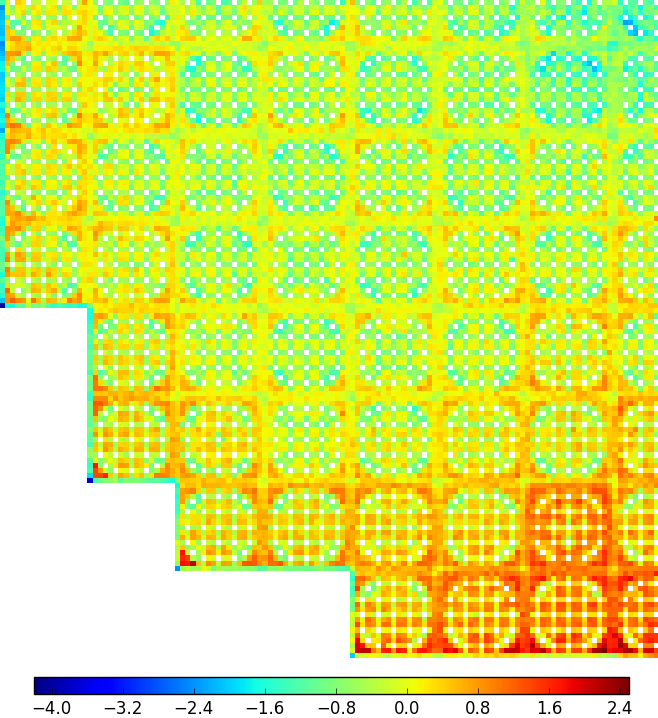
\includegraphics[width=0.65\linewidth]{figures/results/spatial/full-core/capt-err-birch-16}
  \caption{}
  \label{fig:chap11-full-core-capt-err-birch-16}
\end{subfigure}
\caption[U-238 capture rate errors for \ac{BEAVRS}]{U-238 capture percent relative errors for the quarter core \ac{BEAVRS} model with \textit{i}\ac{MGXS} spatial homogenization with BIRCH clustering of 4 (a) and 16 (b) clusters.}
\label{fig:chap11-full-core-capt-err-b}
\end{figure}

\clearpage

SUMMARY BOX

%%%%%%%%%%%%%%%%%%%%%%%%%%%%%%%%%%%%%%%%%%%
\subsubsection{Comparing OpenMOC Solutions}
\label{subsec:chap11-imgxs-capt-rates-compare}

first paragraph: outline
-Fig.~\Crefrange{fig:chap11-assm-1.6-capt-rates-comp}{fig:chap11-assm-refl-capt-rates-comp}
  -individual assemblies and colorsets
  -use the BIRCH clustering scheme for \textit{i}\ac{MGXS} with 2, 4 and 16 clusters
-Fig.~\Crefrange{fig:chap11-assm-full-core-capt-rates-kmeans-comp}{fig:chap11-assm-full-core-capt-rates-birch-comp}
  -full core with $k$-means, \ac{GMM} and BIRCH clustering
-compare errors with null: need equation for what i am displaying here

\begin{equation}
\label{eqn:chap11-compare-openmoc}
\Delta_{k}^{\mathrm{\textit{i}MGXS}} \;\; [\%] \;\; = \;\; \frac{\displaystyle\sum\limits_{g=1}^{G} \hat{\Sigma}^{238}_{\gamma,k,g}\phi_{k,g}^{\mathrm{\textit{i}MGXS}} - \displaystyle\sum\limits_{g=1}^{G} \hat{\Sigma}^{238}_{\gamma,k,g}\phi_{k,g}^{\mathrm{Null}}}{\displaystyle\sum\limits_{g=1}^{G} \hat{\Sigma}^{238}_{\gamma,k,g}\phi_{k,g}^{\mathrm{Null}}} \times 100
\end{equation}

second paragraph: analysis
-can see impact of adding clusters
-2 clusters for a single assm - one cluster for pins adjacent to a \ac{CRGT}
-each new cluster further discriminates local spatial self-shielding effects
  -note 3.1\% assm: 8--16 clusters 
    -discriminates pins both facially and diagonally adjacent to \acp{CRGT}
    -the U-238 capture rates in these pins is largest due to differential moderation from both \acp{CRGT}
-note a few outlier pins in the periodic colorset which break the symmetry
-note the very different clustering for the reflected coloreset
  -first few clusters (2--4) are especially catered to the reflector-assembly and assembly-assembly interfaces
  -later clusters (8--16) are increasingly customized to the more local effects within each assm due to \acp{CRGT} and \acp{BP}
  -illustrates the hierarchical nature of \ac{MGXS} clustering

% note that these plots look different for:
  % 1) each clustering algorithm
  % 2) when dimensionality reduction is used

\begin{figure}[h!]
\centering
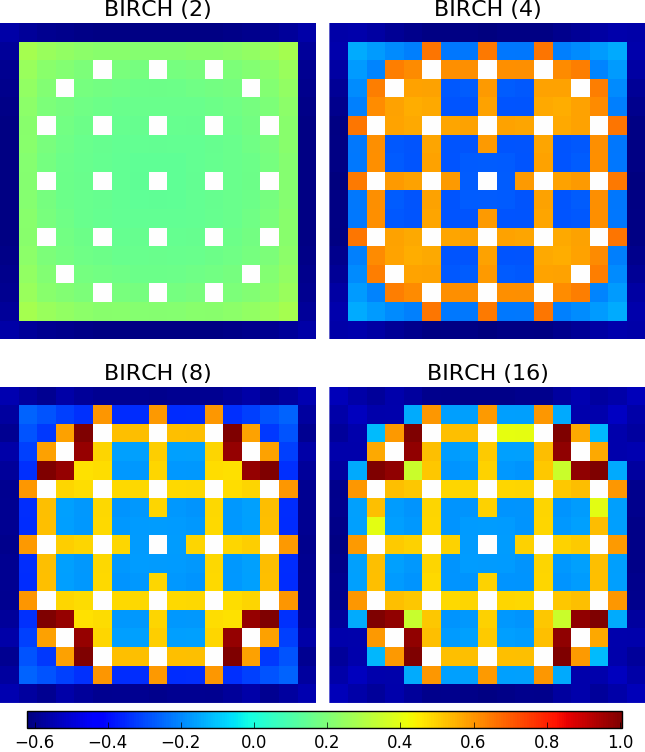
\includegraphics[width=0.9\linewidth]{figures/results/compare/assm-16/compare-capt}
\vspace{2mm}
\caption[U-238 capture rate comparison for a 1.6\% enriched assembly]{A comparison of U-238 capture rate spatial distributions for \textit{i}\ac{MGXS} and null spatial homogenization for a 1.6\% enriched assembly.}
\label{fig:chap11-assm-1.6-capt-rates-comp}
\end{figure}

\clearpage

\begin{figure}[h!]
\centering
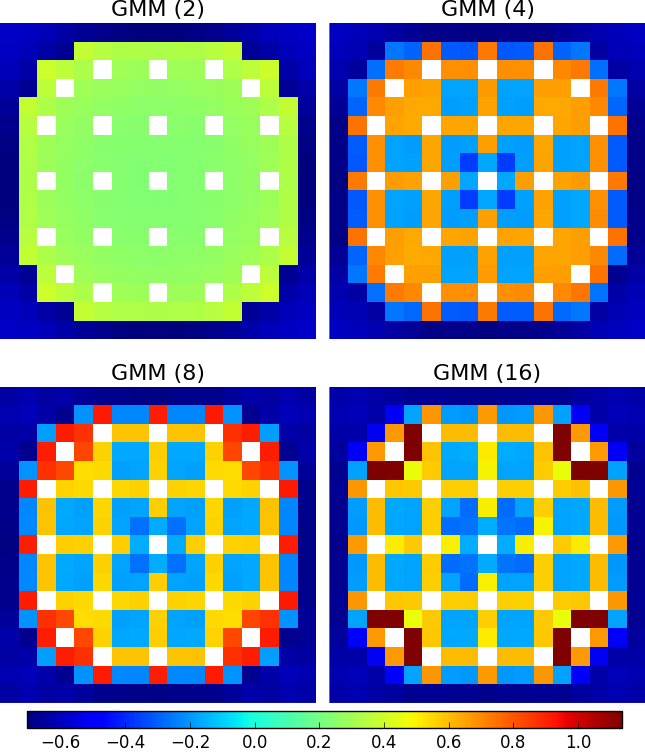
\includegraphics[width=0.9\linewidth]{figures/results/compare/assm-31/compare-capt}
\vspace{2mm}
\caption[U-238 capture rate comparison for a 3.1\% enriched assembly]{A comparison of U-238 capture rate spatial distributions for \textit{i}\ac{MGXS} and null spatial homogenization for a 3.1\% enriched assembly.}
\label{fig:chap11-assm-3.1-capt-rates-comp}
\end{figure}

\clearpage

\begin{figure}[h!]
\centering
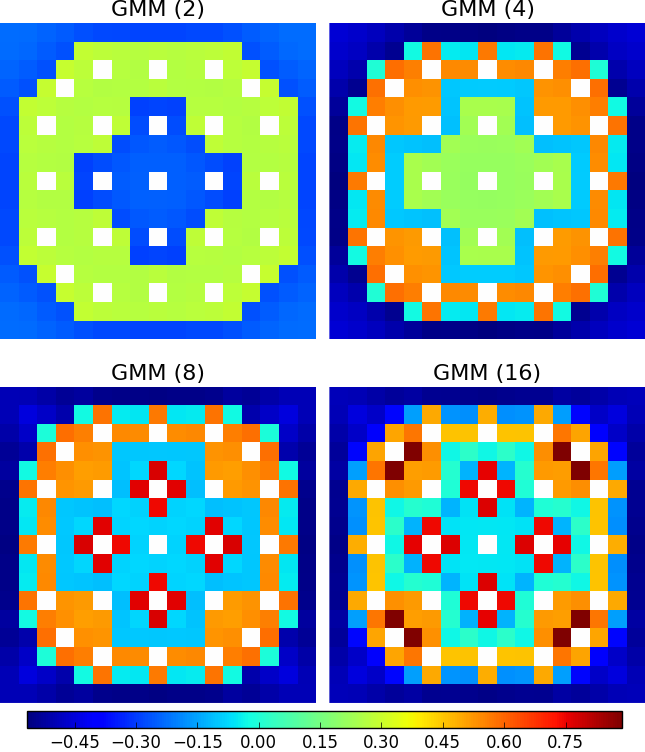
\includegraphics[width=0.9\linewidth]{figures/results/compare/assm-31-20BPs/compare-capt}
\vspace{2mm}
\caption[U-238 capture rate comparison for a 3.1\% enriched assembly with 20 BPs]{A comparison of U-238 capture rate spatial distributions for \textit{i}\ac{MGXS} and null spatial homogenization for a 3.1\% enriched assembly with 20 \acp{BP}.}
\label{fig:chap11-assm-31-20BPs-capt-rates-comp}
\end{figure}
	
\clearpage

\begin{figure}[h!]
\centering
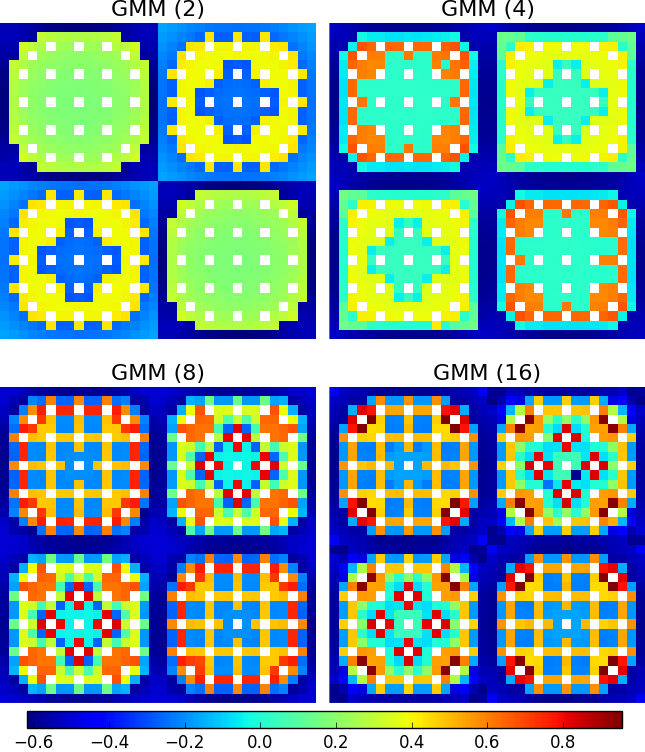
\includegraphics[width=0.9\linewidth]{figures/results/compare/2x2/compare-capt}
\vspace{2mm}
\caption[U-238 capture rate comparison for a 2$\times$2 colorset]{A comparison of U-238 capture rate spatial distributions for \textit{i}\ac{MGXS} and null spatial homogenization for a 2$\times$2 colorset.}
\label{fig:chap11-assm-2x2-capt-rates-comp}
\end{figure}

\clearpage

\begin{figure}[h!]
\centering
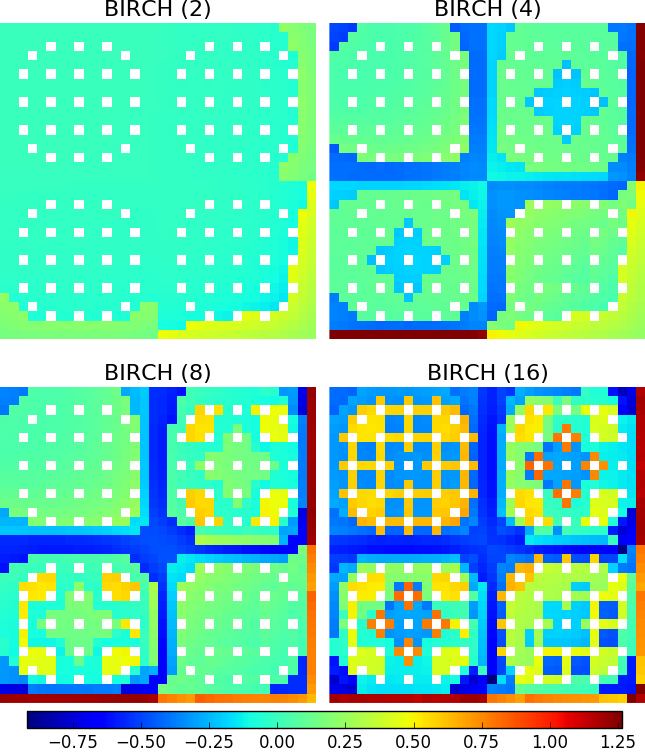
\includegraphics[width=0.9\linewidth]{figures/results/compare/reflector/compare-capt}
\vspace{2mm}
\caption[U-238 capture rate comparison for a 2$\times$2 colorset with reflector]{A comparison of U-238 capture rate spatial distributions for \textit{i}\ac{MGXS} and null spatial homogenization for a 2$\times$2 colorset with a water reflector.}
\label{fig:chap11-assm-refl-capt-rates-comp}
\end{figure}

\clearpage

\begin{figure}[h!]
\centering
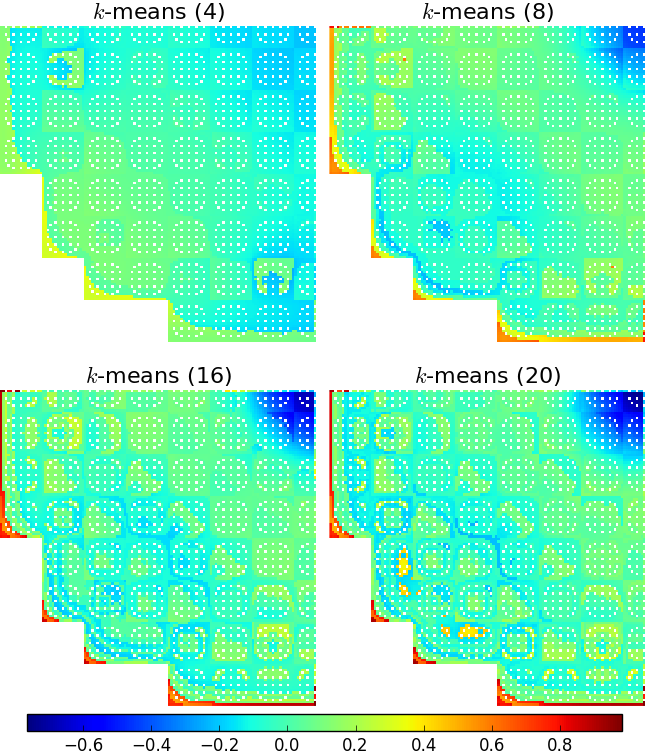
\includegraphics[width=0.9\linewidth]{figures/results/compare/full-core/compare-capt-kmeans}
\vspace{2mm}
\caption[U-238 capture rate comparison for the quarter core BEAVRS model]{A comparison of U-238 capture rate spatial distributions for \textit{i}\ac{MGXS} (\textit{with $k$-means}) and null spatial homogenization for the quarter core BEAVRS model.}
\label{fig:chap11-assm-full-core-capt-rates-kmeans-comp}
\end{figure}

\clearpage

\begin{figure}[h!]
\centering
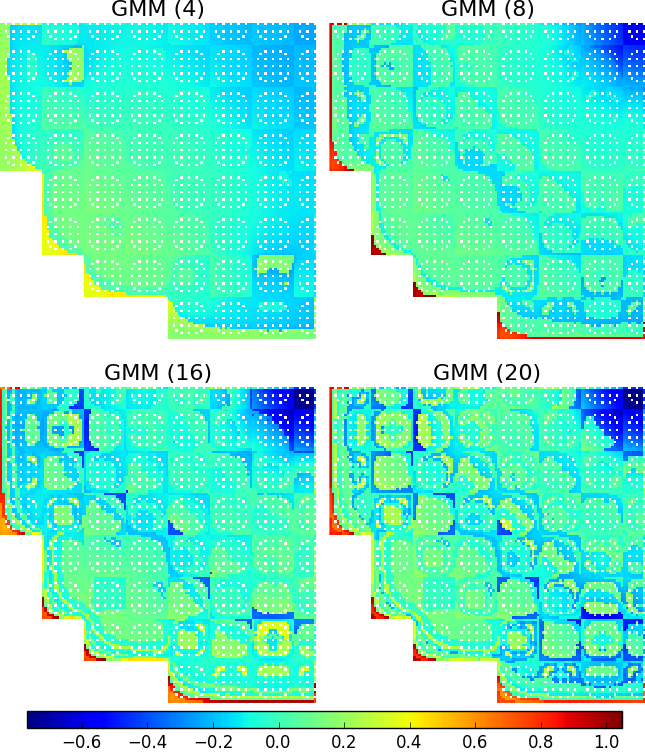
\includegraphics[width=0.9\linewidth]{figures/results/compare/full-core/compare-capt-gmm}
\vspace{2mm}
\caption[U-238 capture rate comparison for the quarter core BEAVRS model]{A comparison of U-238 capture rate spatial distributions for \textit{i}\ac{MGXS} (\textit{with \ac{GMM}}) and null spatial homogenization for the quarter core BEAVRS model.}
\label{fig:chap11-assm-full-core-capt-rates-gmm-comp}
\end{figure}

\clearpage

\begin{figure}[h!]
\centering
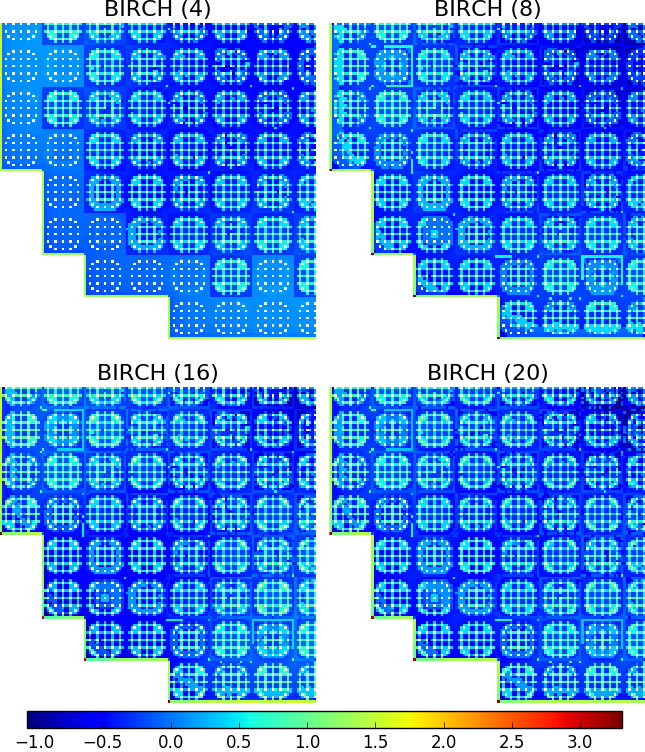
\includegraphics[width=0.9\linewidth]{figures/results/compare/full-core/compare-capt-birch}
\vspace{2mm}
\caption[U-238 capture rate comparison for the quarter core BEAVRS model]{A comparison of U-238 capture rate spatial distributions for \textit{i}\ac{MGXS} (\textit{with BIRCH}) and null spatial homogenization for the quarter core BEAVRS model.}
\label{fig:chap11-assm-full-core-capt-rates-birch-comp}
\end{figure}

\clearpage

SUMMARY BOX


%%%%%%%%%%%%%%%%%%%%%%%%%%%%%%%%%%%%%%%%%%%%%%%%%%%%%%%%%%%%%%%%%%%%%%%%%%%%%%%
\section{Performance with Converged MGXS}
\label{sec:chap11-converge}

first paragraph: objective
-want to evaluate how quickly OpenMOC solutions converge
-how many particle histories are needed to sufficiently converge \ac{MGXS} for converged OpenMOC solutions?
  -for null, degenerate and \textit{i}\ac{MGXS} spatial homogenization schemes?
-perfect batchwise: how much ``noise'' can we live with in our tally data???
  -perform clustering on most highly converged \ac{MGXS} data
  -(re-use) the same cluster model for ``noisier'' \ac{MC} tally data
  -provides a means to answer the thought experiment: if I could find the ``perfect'' clustering from ``noisy'' data, how accurate could my OpenMOC solutions be?
-also want to compare statistical uncertainty of OpenMC solutions for each statepoint
  -alternative to run reference OpenMC in place of deterministic multi-group code

second paragraph: runtime params
-100,000 particles / batch - individual assemblies
-100,000 particles / batch - 2x2 and reflector??
%-1,000,000 particles / batch - quarter core
-10,000 batches for assemblies and reflector (100 inactive)
%-how many for full core??
-reported statepoints for 100 logarithmically spaced batches
  -80\% of statepoints in first 10 -- 1000 active batches (1 -- 100 million histories)
  -20\% of statepoints in latter 1000 -- 9800 active batches (100 -- nearly 1 billion histories)

third paragraph: outline
-Sec.~\ref{subsec:chap11-eigenvalue-converge} - convergence of the eigenvalues
-Sec.~\ref{subsec:chap11-capture-converge} - convergence of U-238 capture rate relative errors

%%%%%%%%%%%%%%%%%%%%%%%%%%%%%%%%%%%
\subsection{Eigenvalue Convergence}
\label{subsec:chap11-eigenvalue-converge}

first paragraph: outline
-Figs.~\Crefrange{fig:chap11-assm-1.6-eigenvalue-converge}{fig:chap11-refl-eigenvalue-converge}
  -individual assemblies and colorsets
-use BIRCH clustering with 2, 4 and 10 clusters for assemblies and periodic colorset
-use BIRCH clustering with 2, 4 and 16 clusters for reflected colorset

second paragraph: analysis
-all cluster models converge to the same eigenvalue bias
  -null and \textit{i}\ac{MGXS} schemes quite consistent
  -degenerat scheme diverges up to 100 \ac{pcm} but eventually converges with the other two
-bias fluctuates on the order of 500 \ac{pcm} with fewer than 10$^{7}$ histories
-requires on the order of 10$^{8}$ histories to converge the eigenvalue bias
  -EVEN for null homogenization!!!
-WHY??:
  -uncertainties on MGXS
  -difference between track-length and analog estimated MGXS
    -this builds in an inherent bias for few particle histories
    -reference Nelson~\cite{nelson2014improved}

\begin{figure}[h!]
\centering
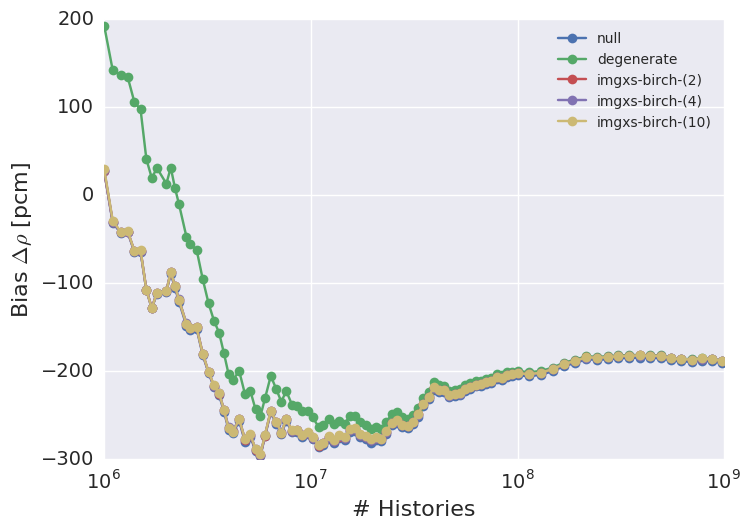
\includegraphics[width=0.87\linewidth]{figures/results/convergence/assm-16/keff-bias-evo}
\vspace{2mm}
\caption[Eigenvalue bias covergence for a 1.6\% enriched assembly]{Convergence of the eigenvalue bias $\Delta\rho$ for a 1.6\% enriched assembly.}
\label{fig:chap11-assm-1.6-eigenvalue-converge}
\end{figure}

\begin{figure}[h!]
\centering
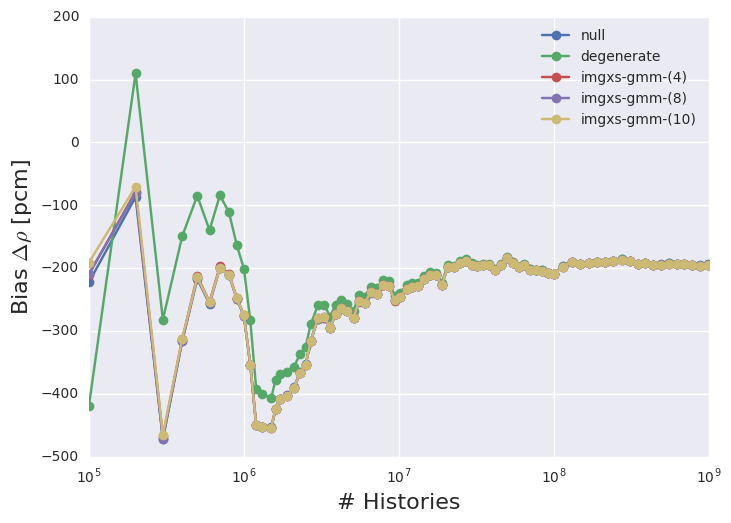
\includegraphics[width=0.87\linewidth]{figures/results/convergence/assm-31/keff-bias-evo}
\vspace{2mm}
\caption[Eigenvalue bias covergence for a 3.1\% enriched assembly]{Convergence of the eigenvalue bias $\Delta\rho$ for a 3.1\% enriched assembly.}
\label{fig:chap11-assm-3.1-eigenvalue-converge}
\end{figure}

\begin{figure}[h!]
\centering
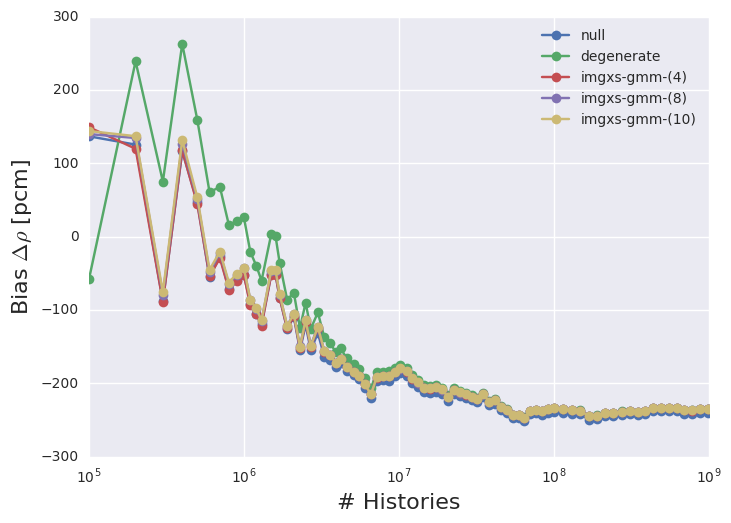
\includegraphics[width=0.87\linewidth]{figures/results/convergence/assm-31-20BPs/keff-bias-evo}
\vspace{2mm}
\caption[Eigenvalue bias covergence for a 3.1\% enriched assembly with 20 \acp{BP}]{Convergence of the eigenvalue bias $\Delta\rho$ for a 3.1\% enriched assembly with 20 \acp{BP}.}
\label{fig:chap11-assm-3.1-20BPs-eigenvalue-converge}
\end{figure}

\begin{figure}[h!]
\centering
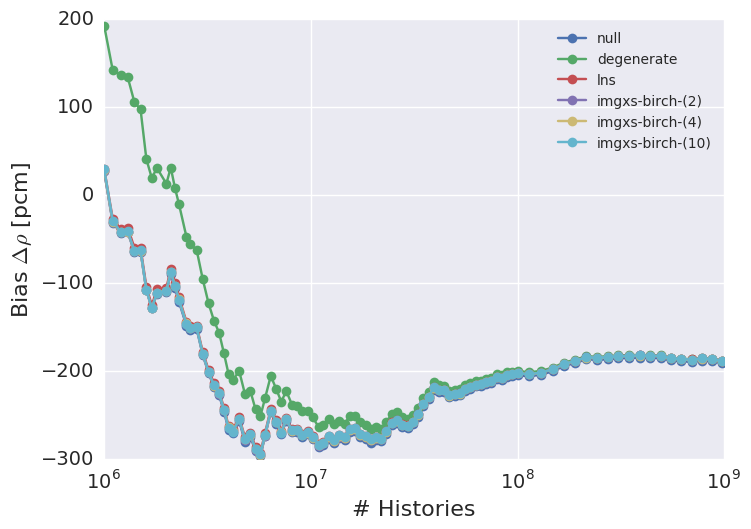
\includegraphics[width=0.87\linewidth]{figures/results/convergence/2x2/keff-bias-evo}
\vspace{2mm}
\caption[Eigenvalue bias covergence for a 2$\times$2 colorset]{Convergence of the eigenvalue bias $\Delta\rho$ for a 2$\times$2 colorset.}
\label{fig:chap11-2x2-eigenvalue-converge}
\end{figure}

\begin{figure}[h!]
\centering
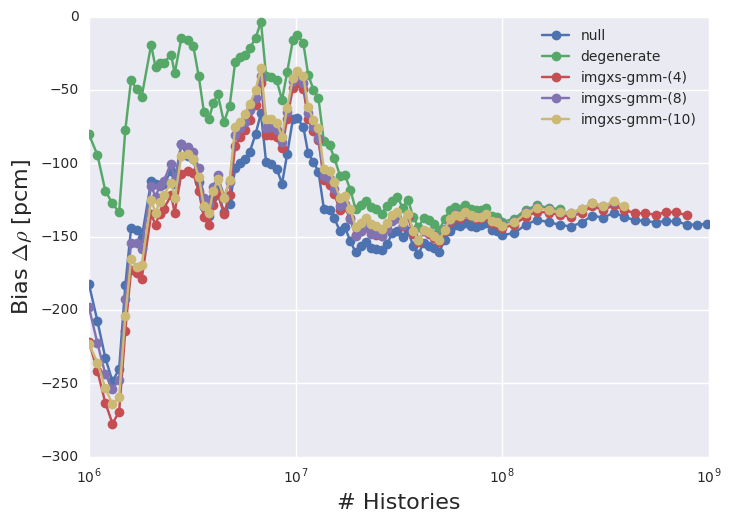
\includegraphics[width=0.87\linewidth]{figures/results/convergence/reflector/keff-bias-evo}
\vspace{2mm}
\caption[Eigenvalue bias covergence for a 2$\times$2 colorset with reflector]{Convergence of the eigenvalue bias $\Delta\rho$ for a 2$\times$2 colorset with a water reflector.}
\label{fig:chap11-refl-eigenvalue-converge}
\end{figure}

-plots for full core

SUMMARY BOX

%%%%%%%%%%%%%%%%%%%%%%%%%%%%%%%%%%%%%%%%%%%
\subsection{U-238 Capture Rate Convergence}
\label{subsec:chap11-capture-converge}

first paragraph: outline
-Figs.~\Crefrange{fig:chap11-assm-1.6-capture-converge}{fig:chap11-refl-capture-converge}
  -individual assemblies and colorsets
-use BIRCH clustering with 2, 4 and 10 clusters for assemblies and periodic colorset
-use BIRCH clustering with 2, 4 and 16 clusters for reflected colorset
-openmc 1-sigma uncertainty is reported relative to the mean
  -not a direct comparison to the percentage relative error reported for OpenMOC

second paragraph: analysis
-smoother convergence for mean than for the max error
-openmc will converge to zero
-null, degenerate and \textit{i}\ac{MGXS} schemes will not converge to some non-zero bias
  -accounts for various approx (energy, spatial and angular discretization)
-convergence of null
  -null is stable with 100,000 particles for assemblies and 1,000,000 particle for colorsets
-convergence of degenerate
  -takes over 100,000,000 particles to converge for assemblies
  -takes at least 1,000,000,000 particles to converge for colorsets (not even shown on plots)
-convergence of \textit{i}\ac{MGXS}
  -the more clusters, the longer it takes to converge
  -the more clusters, the lower the final converged value (smaller bias)
  -the more clusters, the more erratic the convergence
    -would be interesting to look at alternatives to track density-weighting
    -how about taking the median MGXS from each cluster?
      -would be less sensitive to outliers and potentially more ``robust''
      -but wouldn't preserve global reactivity
    -recall argument about LNS - uneven number of fuel pin instances assigned to each cluster
      -clusters with the fewest pins will be most constraining on convergence
-convergence of openmc to degenerate
  -openmc max always less than degenerate
  -but openmc mean greater than degenerate for few particles
    -eventually drops below as degenerate converges to non-zero bias
  -takes perhaps 30,000,000 particles for max to reach degenerate for assemblies (60,000,000 for colorsets?)
  -but over 500,000,000 particles for mean to reach degenerate

\begin{figure}[h!]
\centering
\begin{subfigure}{\textwidth}
  \centering
  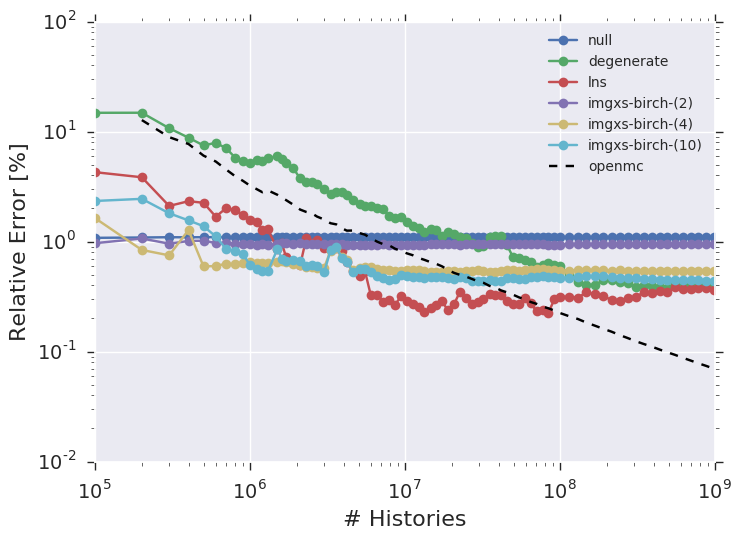
\includegraphics[width=0.9\linewidth]{figures/results/convergence/assm-16/max-capt-err-evo}
  \caption{}
  \label{fig:chap11-assm-1.6-capture-converge-max}
\end{subfigure}
\begin{subfigure}{\textwidth}
  \centering
  \includegraphics[width=0.9\linewidth]{figures/results/convergence/assm-16/mean-capt-err-evo}
  \caption{}
  \label{fig:chap11-assm-1.6-capture-converge-mean}
\end{subfigure}
\vspace{2mm}
\caption[Fission rate covergence for a 1.6\% enriched assembly]{Convergence of the max (a) and mean (b) absolute U-238 capture rate percent relative errors for a 1.6\% enriched assembly.}
\label{fig:chap11-assm-1.6-capture-converge}
\end{figure}

\begin{figure}[h!]
\centering
\begin{subfigure}{\textwidth}
  \centering
  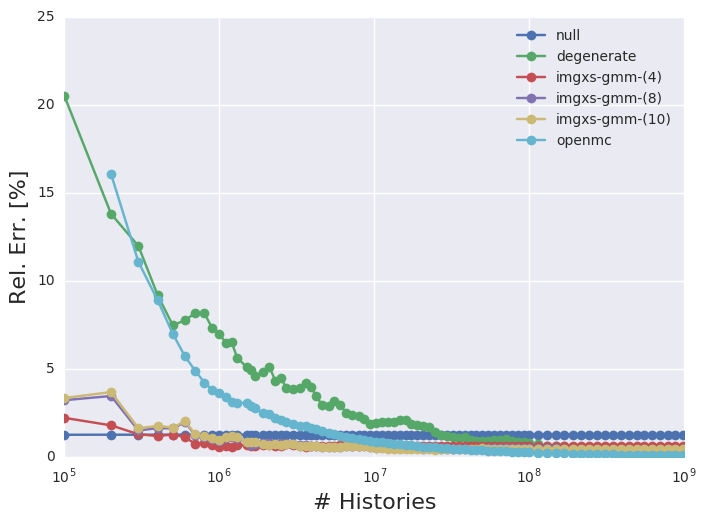
\includegraphics[width=0.9\linewidth]{figures/results/convergence/assm-31/max-capt-err-evo}
  \caption{}
  \label{fig:chap11-assm-3.1-capture-converge-max}
\end{subfigure}
\begin{subfigure}{\textwidth}
  \centering
  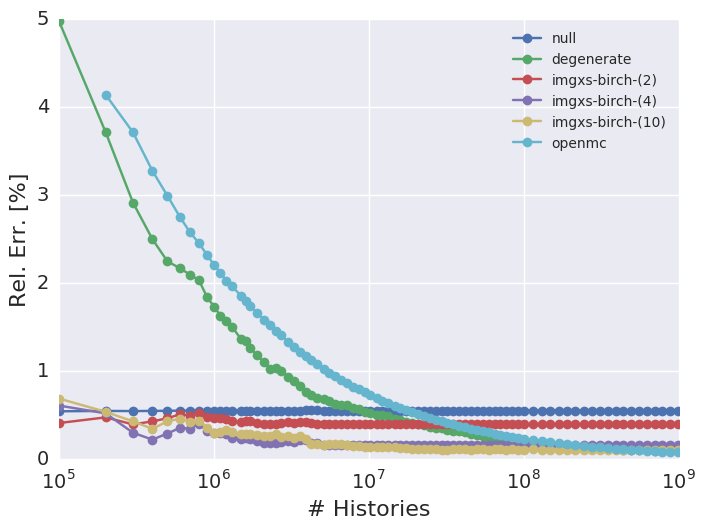
\includegraphics[width=0.9\linewidth]{figures/results/convergence/assm-31/mean-capt-err-evo}
  \caption{}
  \label{fig:chap11-assm-3.1-capture-converge-mean}
\end{subfigure}
\vspace{2mm}
\caption[Fission rate covergence for a 3.1\% enriched assembly]{Convergence of the max (a) and mean (b) absolute U-238 capture rate percent relative errors for a 3.1\% enriched assembly.}
\label{fig:chap11-assm-3.1-capture-converge}
\end{figure}

\begin{figure}[h!]
\centering
\begin{subfigure}{\textwidth}
  \centering
  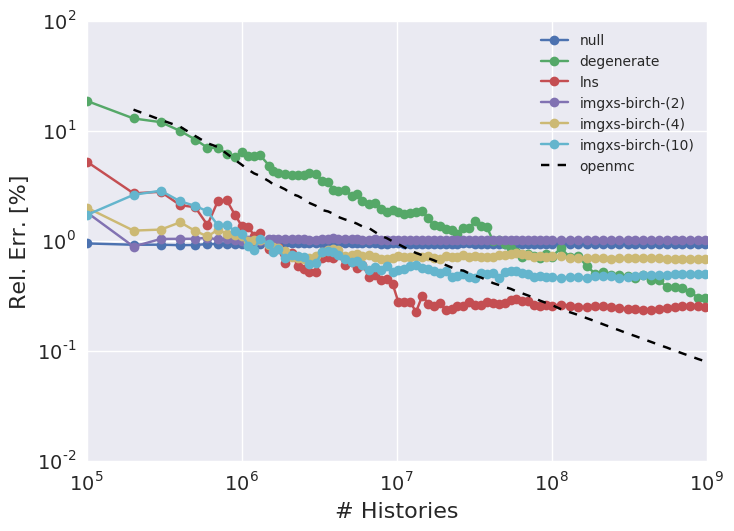
\includegraphics[width=0.9\linewidth]{figures/results/convergence/assm-31-20BPs/max-capt-err-evo}
  \caption{}
  \label{fig:chap11-assm-3.1-20BPs-capture-converge-max}
\end{subfigure}
\begin{subfigure}{\textwidth}
  \centering
  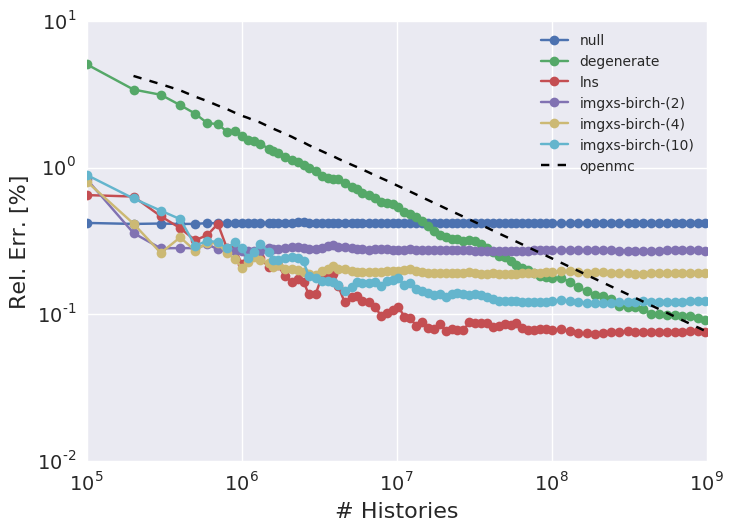
\includegraphics[width=0.9\linewidth]{figures/results/convergence/assm-31-20BPs/mean-capt-err-evo}
  \caption{}
  \label{fig:chap11-assm-3.1-20BPs-capture-converge-mean}
\end{subfigure}
\vspace{2mm}
\caption[Fission rate covergence for a 3.1\% enriched assembly with 20 \acp{BP}]{Convergence of the max (a) and mean (b) absolute U-238 capture rate percent relative errors for a 3.1\% enriched assembly with 20 \acp{BP}.}
\label{fig:chap11-assm-3.1-20BPs-capture-converge}
\end{figure}

\begin{figure}[h!]
\centering
\begin{subfigure}{\textwidth}
  \centering
  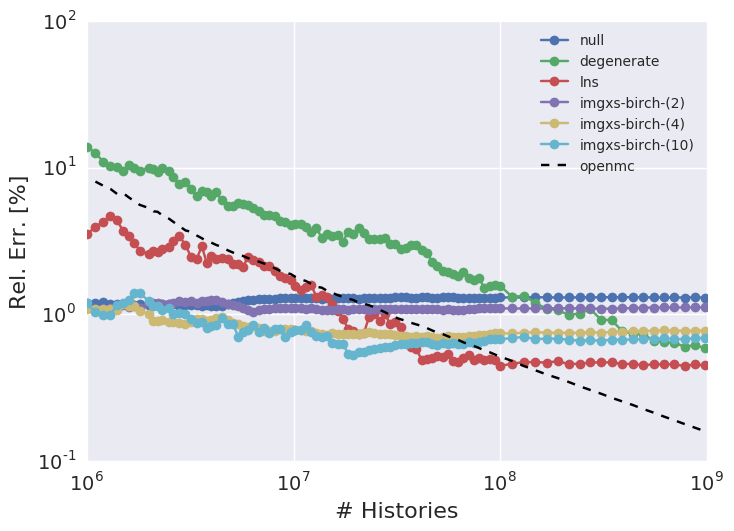
\includegraphics[width=0.9\linewidth]{figures/results/convergence/2x2/max-capt-err-evo}
  \caption{}
  \label{fig:chap11-2x2-capture-converge-max}
\end{subfigure}
\begin{subfigure}{\textwidth}
  \centering
  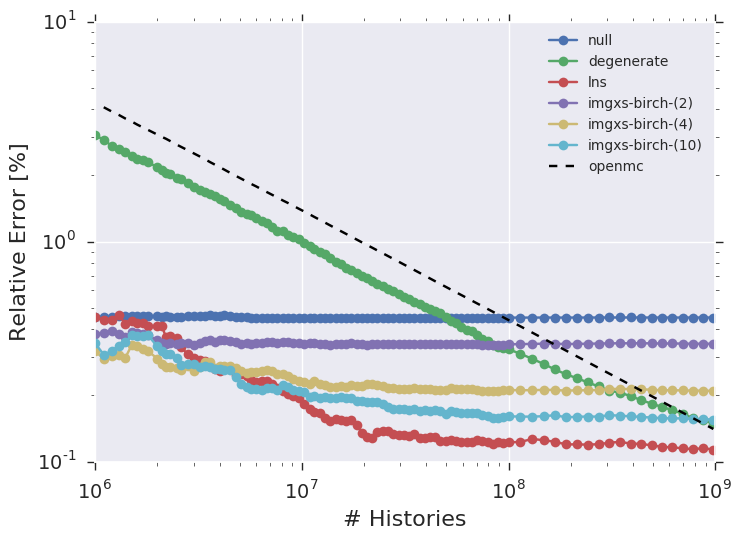
\includegraphics[width=0.9\linewidth]{figures/results/convergence/2x2/mean-capt-err-evo}
  \caption{}
  \label{fig:chap11-2x2-capture-converge-mean}
\end{subfigure}
\vspace{2mm}
\caption[Fission rate covergence for a 2$\times$2 colorset]{Convergence of the max (a) and mean (b) absolute U-238 capture rate percent relative errors for a 2$\times$2 colorset.}
\label{fig:chap11-2x2-capture-converge}
\end{figure}

\begin{figure}[h!]
\centering
\begin{subfigure}{\textwidth}
  \centering
  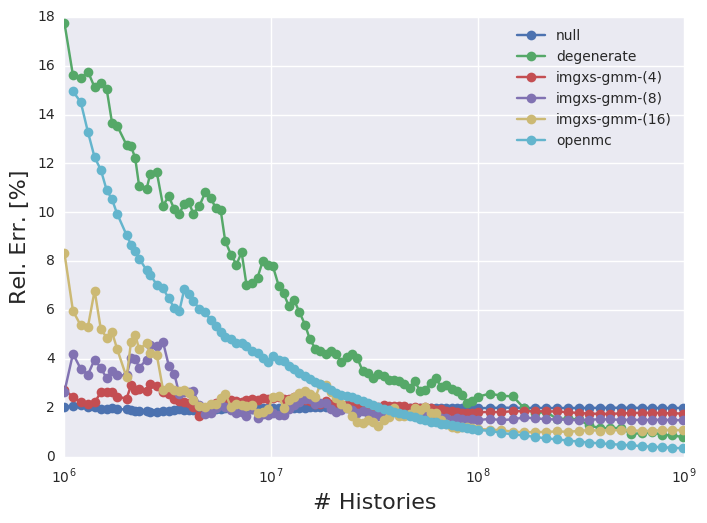
\includegraphics[width=0.9\linewidth]{figures/results/convergence/reflector/max-capt-err-evo}
  \caption{}
  \label{fig:chap11-refl-capture-converge-max}
\end{subfigure}
\begin{subfigure}{\textwidth}
  \centering
  \includegraphics[width=0.9\linewidth]{figures/results/convergence/reflector/mean-capt-err-evo}
  \caption{}
  \label{fig:chap11-refl-capture-converge-mean}
\end{subfigure}
\vspace{2mm}
\caption[Fission rate covergence for a 2$\times$2 colorset with reflector]{Convergence of the max (a) and mean (b) absolute U-238 capture rate percent relative errors for a 2$\times$2 colorset with a water reflector.}
\label{fig:chap11-refl-capture-converge}
\end{figure}

-full core plots

SUMMARY BOX


%%%%%%%%%%%%%%%%%%%%%%%%%%%%%%%%%%%%%%%%%%%%%%%%%%%%%%%%%%%%%%%%%%%%%%%%%%%%%%%
\section{Evaluation of Model Selection Techniques}
\label{sec:chap11-model-select}

first paragraph: objective
-recall Sec.~\ref{sec:chap10-model-select}
-model selection needed to select number of clusters
  -can only evaluate clustering models with respect to the \ac{MC} tally data
  -don't have access to either:
    1) the ``true'' cluster labels
    2) the OpenMOC-OpenMC error
-can use intra-cluster and inter-cluster similarities
-can use likelihood and regularization (BIC) to balance bias-variance tradeoff

second paragraph: outline
-evaluate each heuristic with the 1.6\% enr assm and 2$\times$2 colorset with water reflector
-Sec.~\ref{subsec:chap11-db-index} Davies-Bouldin indices
-Sec.~\ref{subsec:chap11-dunn-index} Dunn indices
-Sec.~\ref{subsec:chap11-ch-index} Calinski-Harabaz indices
-Sec.~\ref{subsec:chap11-silhouette-coeff} silhouette coefficients
-Sec.~\ref{subsec:chap11-bic} Bayesian Information Criterion

-consider that cross-validation could make these heuristics more robust and less erratic
  -recall Sec.~\ref{subsec:chap10-cross-validate}
-could compare cluster labels to those from LNS (use LNS as the ``ground truth'')
-make axes labels clearer

%%%%%%%%%%%%%%%%%%%%%%%%%%%%%%%%%
\subsection{Davies-Bouldin Index}
\label{subsec:chap11-db-index}

first paragraph: outline and analysis
-recall Sec.~\ref{subsec:chap10-db-index}
-Figs.~\Crefrange{fig:chap11-assm-16-db-index}{fig:chap11-refl-db-index}
-want to minimize DB index
-minima are all for a single cluster
-can use ``elbow'' method to look at point at which DB index shoots up
  -around 10 clusters for assm
  -around 9 clusters for colorset
-not clear how one would use these results to create a robust, automated model selection system
  -perhaps CV would help??

\begin{figure}[h!]
\centering
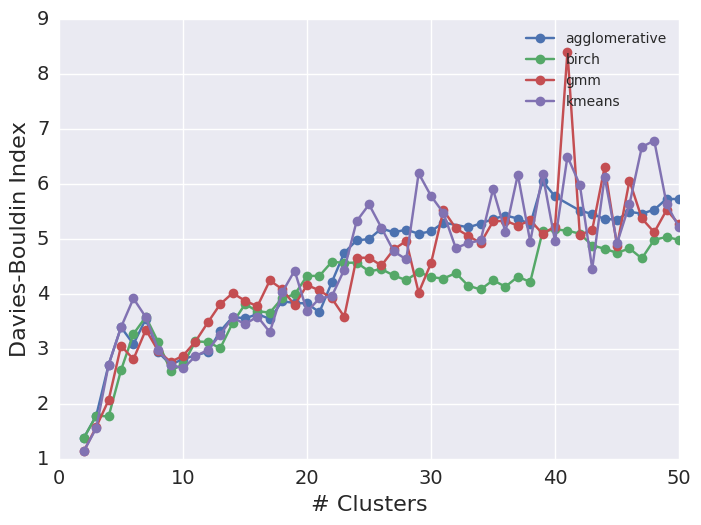
\includegraphics[width=0.87\linewidth]{figures/results/model-select/assm-16/db-combined-U238-capture-1}
\vspace{2mm}
\caption[Davies-Bouldin indices for the 1.6\% enriched assembly]{Davies-Bouldin indices for the 1.6\% enriched assembly.}
\label{fig:chap11-assm-16-db-index}
\end{figure}

\begin{figure}[h!]
\centering
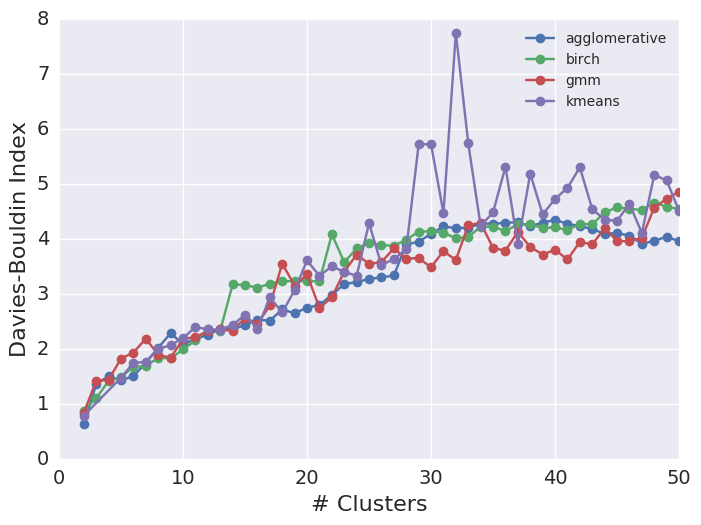
\includegraphics[width=0.87\linewidth]{figures/results/model-select/reflector/db-combined-U238-nu-fission-1}
\vspace{2mm}
\caption[Davies-Bouldin indices for the 2$\times$2 colorset with reflector]{Davies-Bouldin indices for the 2$\times$2 colorset with a water reflector.}
\label{fig:chap11-refl-db-index}
\end{figure}

%%%%%%%%%%%%%%%%%%%%%%%
\subsection{Dunn Index}
\label{subsec:chap11-dunn-index}

first paragraph: outline and analysis
-recall Sec.~\ref{subsec:chap10-dunn-index}
-Figs.~\Crefrange{fig:chap11-assm-16-dunn-index}{fig:chap11-refl-dunn-index}
-want to maximize Dunn index
-Dunn index is constrained by the most poorly behaving cluster
  -leads to the step-like behavior
    -indicates that the most poorly behaving cluster is not always refined with each successive cluster added to the models
-again not clear how one would use these results to create a robust, automated model selection system
  -perhaps CV would help??

\begin{figure}[h!]
\centering
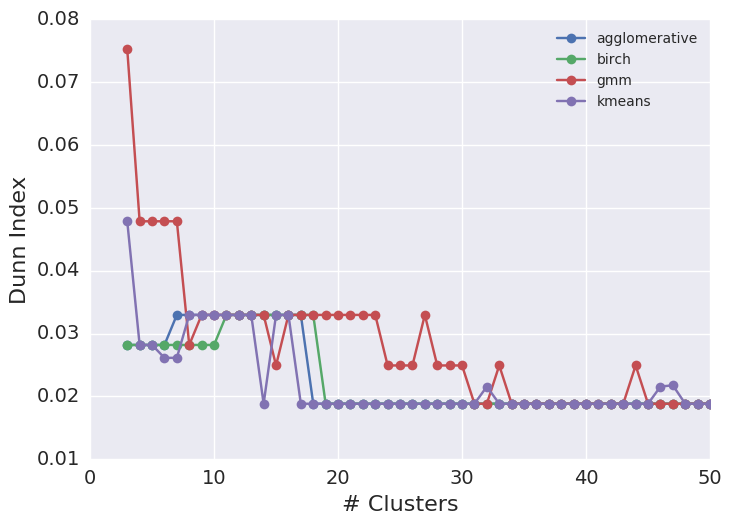
\includegraphics[width=0.87\linewidth]{figures/results/model-select/assm-16/dunn-combined-U238-capture-1}
\vspace{2mm}
\caption[Dunn indices for the 1.6\% enriched assembly]{Dunn indices for the 1.6\% enriched assembly.}
\label{fig:chap11-assm-16-dunn-index}
\end{figure}

\begin{figure}[h!]
\centering
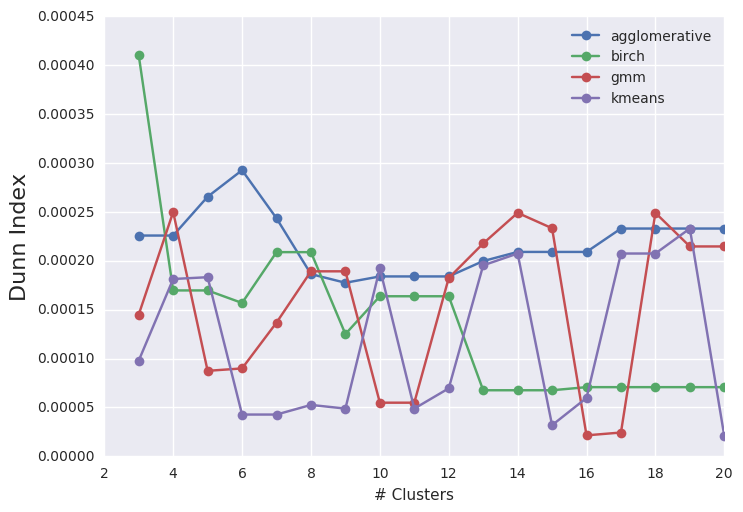
\includegraphics[width=0.87\linewidth]{figures/results/model-select/reflector/dunn-combined-U238-nu-fission-1}
\vspace{2mm}
\caption[Dunn indices for the 2$\times$2 colorset with reflector]{Dunn indices for the 2$\times$2 colorset with a water reflector.}
\label{fig:chap11-refl-dunn-index}
\end{figure}

%%%%%%%%%%%%%%%%%%%%%%%%%%%%%%%%%%%
\subsection{Calinski-Harabaz Index}
\label{subsec:chap11-ch-index}

first paragraph: outline and analysis
-recall Sec.~\ref{subsec:chap10-calinski-harabaz}
-Figs.~\Crefrange{fig:chap11-assm-16-ch-index}{fig:chap11-refl-ch-index}
-want to maximize CH index
-more smoothly varying behavior
-more tightly bunched behavior for the four algorithms than was the case for Dunn and DB
-index doesn't seem to peak at 20 clusters for CH index
-seems to reach plateau after 10 -- 14 clusters for colorset
-again not clear how one would use these results to create a robust, automated model selection system
  -perhaps CV would help??

\begin{figure}[h!]
\centering
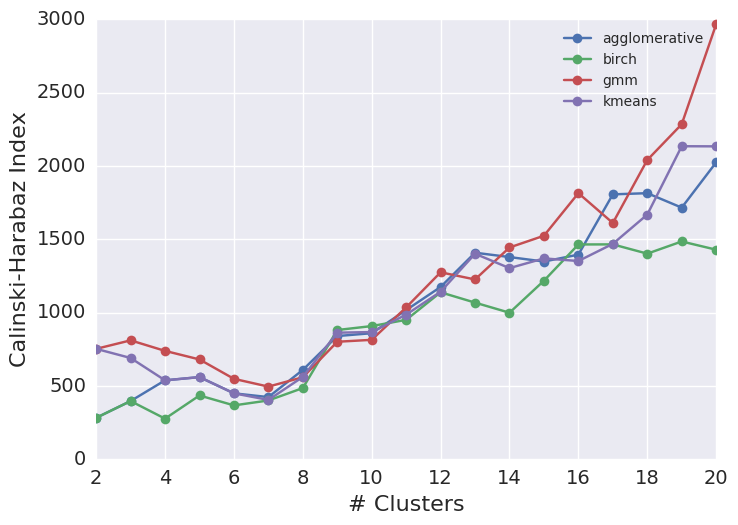
\includegraphics[width=0.87\linewidth]{figures/results/model-select/assm-16/ch-combined-U238-capture-1}
\vspace{2mm}
\caption[Calinski-Harabaz indices for the 1.6\% enriched assembly]{Calinski-Harabaz indices for the 1.6\% enriched assembly.}
\label{fig:chap11-assm-16-ch-index}
\end{figure}

\begin{figure}[h!]
\centering
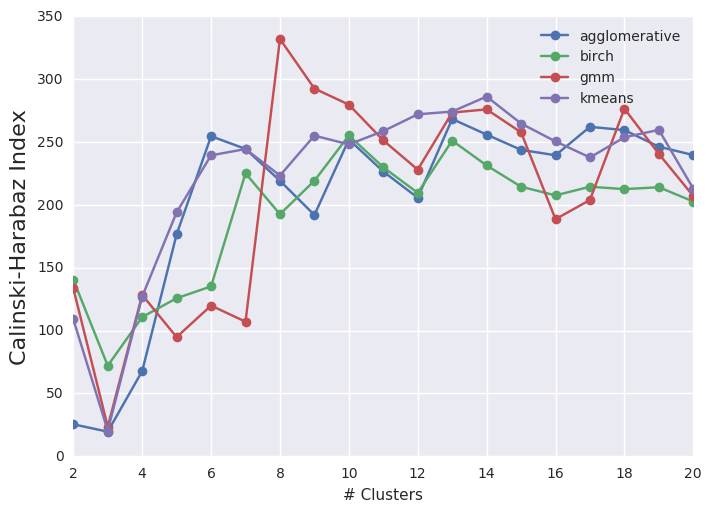
\includegraphics[width=0.87\linewidth]{figures/results/model-select/reflector/ch-combined-U238-nu-fission-1}
\vspace{2mm}
\caption[Calinski-Harabaz indices for the 2$\times$2 colorset with reflector]{Calinski-Harabaz indices for the 2$\times$2 colorset with a water reflector.}
\label{fig:chap11-refl-ch-index}
\end{figure}

%%%%%%%%%%%%%%%%%%%%%%%%%%%%%%%%%%%
\subsection{Silhouette Coefficient}
\label{subsec:chap11-silhouette-coeff}

first paragraph: outline and analysis
-recall Sec.~\ref{subsec:chap10-silhouette-coeff}
-Figs.~\Crefrange{fig:chap11-assm-16-silhouette-coeff}{fig:chap11-refl-silhouette-coeff}
-want to maximize silhouette coeff
-coeffs peak for a single cluster for both assm and colorset
-more tightly bunched behavior for the four algorithms than was the case for Dunn and DB, but less so than for CH
-again not clear how one would use these results to create a robust, automated model selection system
  -perhaps CV would help??

\begin{figure}[h!]
\centering
\includegraphics[width=0.87\linewidth]{figures/results/model-select/assm-16/silhouette-combined-U238-capture-1}
\vspace{2mm}
\caption[Silhouette coefficients for the 1.6\% enriched assembly]{Silhouette coefficients for the 1.6\% enriched assembly.}
\label{fig:chap11-assm-16-silhouette-coeff}
\end{figure}

\begin{figure}[h!]
\centering
\includegraphics[width=0.87\linewidth]{figures/results/model-select/reflector/silhouette-combined-U238-nu-fission-1}
\vspace{2mm}
\caption[Silhouette coefficients for the 2$\times$2 colorset with reflector]{Silhouette coefficients for the 2$\times$2 colorset with a water reflector.}
\label{fig:chap11-refl-silhouette-coeff}
\end{figure}

%%%%%%%%%%%%%%%%%%%%%%%%%%%%%%%%%%%%%%%%%%%
\subsection{Bayesian Information Criterion}
\label{subsec:chap11-bic}

first paragraph: outline and analysis
-recall Sec.~\ref{subsec:chap10-bic}
-Figs.~\Crefrange{fig:chap11-assm-16-bic}{fig:chap11-refl-bic}
-want to minimize BIC
-BIC only has closed form solution for \ac{GMM}
-BIC is much more smoothly varying with the number of clusters than the preceding metrics
-BIC doesn't seem to reach a minima even with 20 clusters
  -though seems to be leveling for the single assm
  -would eventually start to increase due to growth of second penalty term in the BIC expression
-can see the impact of diminishing returns in the BIC
  -the first 5 clusters causes the BIC to decrease the most
-could foresee a method which would choose the number of clusters using this method
  -might choose based on the fractional change in the BIC with each successive cluster

\begin{figure}[h!]
\centering
\includegraphics[width=0.87\linewidth]{figures/results/model-select/assm-16/bic-combined-U238-capture-1}
\vspace{2mm}
\caption[Silhouette coefficients for the 1.6\% enriched assembly]{Bayesian Information Criteria (BIC) for the 1.6\% enriched assembly.}
\label{fig:chap11-assm-16-bic}
\end{figure}

\begin{figure}[h!]
\centering
\includegraphics[width=0.87\linewidth]{figures/results/model-select/reflector/bic-combined-U238-nu-fission-1}
\vspace{2mm}
\caption[BIC for the 2$\times$2 colorset with reflector]{Bayesian Information Criteria (BIC) for the 2$\times$2 colorset with a water reflector.}
\label{fig:chap11-refl-bic}
\end{figure}

SUMMARY BOX!!!

%%%%%%%%%%%%%%%%%%%%%%%%%%%%%%%%%%%%%%%%%%%%%%%%%%%%%%%%%%%%%%%%%%%%%%%%%%%%%%%
\section{Synthesis}
\label{sec:chap11-synthesis}

first paragraph:
-bring it all together - what does it all mean??
  -refer to Fig.~\ref{fig:chap10-flow-chart}
  -recall dual goals - runtime, MC accuracy, etc.
-quantify how much faster \textit{i}\ac{MGXS} would be then full core MC
  -Tab.~\ref{table:chap11-runtimes}
-OpenMOC runtimes for litmus-only feature selection with ? with ? clusters

second paragraph:
-refer to Kord's suggestions about comparing to case where each individual sub-component is modeled
 -each unique assm
 -each colorset
 -corner-baffle case

-define a Figure of merit per Kord's suggestion
-add rel. err. and uncertainty to the table

%OpenMC particles / sec / core
%benchmark         no MGXs        MGXS
%1.6               2673.3         1154.4
%3.1               3012.9         1265.1
%3.1 BPs           3051.4         1011.4
%2x2               2976.3          784.9
%reflector         3004.6          795.6
%quarter core      2361.5          622.2

-use particle tracking rate to compute total time
  -read number of batches from the convergence plots as the max(max err,mean err) <= degenerate err
  -multiply number of batches by particle tracking rate
  -this uses the tracking rate without MGXS for the ``reference''
  -this use the tracking rate with MGXS for all others
  -10 clusters each???

\begin{table}[ht!]
  \centering
  \caption[Computational resource requirements for each simulation approach]{The computational resources needed for various simulation approaches to reach the level of accuracy achieved with degenerate spatial homogenization.}
  \small
  \label{table:chap11-runtimes}
  \vspace{6pt}
  \begin{tabular}{l l R{2.5cm} R{1.5cm} S[table-format=3.2] S[table-format=3.2] S[table-format=3.2]}
  \toprule
  \rowcolor{lightgray}
  & & & \multicolumn{3}{c}{\cellcolor{lightgray} \bf Runtime [core-hours]} \\
  \multirow{-2}{*}{\cellcolor{lightgray} \bf Benchmark} &
  \multirow{-2}{*}{\cellcolor{lightgray} \bf Scheme} &
  \multirow{-2}{*}{\cellcolor{lightgray} \bf \# Particles} &
  \multirow{-2}{*}{\cellcolor{lightgray} \bf Rel. Err. [\%]} &
  \multicolumn{1}{c}{\cellcolor{lightgray} \bf OpenMC} &
  \multicolumn{1}{c}{\cellcolor{lightgray} \bf OpenMOC} &
  \multicolumn{1}{c}{\cellcolor{lightgray} \bf Total} \\
  \midrule
\multirow{4}{*}{\parbox{2.5cm}{1.6\% Assm}} & Reference & 550,000,000 & & 57.2 & & 57.2 \\
& Null & 100,000 & &  0.02 & 0.36 & 0.38 \\
& Degenerate & 115,000,000 & & 27.7 & 0.40 & 28.1 \\
& \textit{i}\ac{MGXS} & 4,000,000 & & 0.96 & 0.38 & 1.34 \\
  \midrule
\multirow{4}{*}{\parbox{2.5cm}{3.1\% Assm}} & Reference & 550,000,000 & & 50.7 & & 50.7 \\
& Null & 100,000 & & 0.02 & 0.40 & 0.42 \\
& Degenerate & 115,000,000 & & 25.3 & 0.40 & 25.7 \\
& \textit{i}\ac{MGXS} & 4,000,000 & & 0.88 & 0.37 & 1.25 \\
  \midrule
\multirow{4}{*}{\parbox{2.5cm}{3.1\% Assm w/ 20 \acp{BP}}} & Reference & 550,000,000 & & 50.1 & & 50.1 \\
& Null & 100,000 & & 0.02 & 0.41 & 0.43 \\
& Degenerate & 115,000,000 & & 27.7 & 0.41 & 28.1 \\
& \textit{i}\ac{MGXS} & 4,000,000 & & 0.96 & 0.42 & 1.38 \\
  \midrule
\multirow{4}{*}{\parbox{2.5cm}{2$\times$2 Colorset}} & Reference & 8,755,000 & & 81.7 & & 81.7 \\
& Null & 100,000 & & 0.04 & 2.00 & 2.03 \\
& Degenerate & 700,000,000 & & 248 & 2.29 & 250 \\
& \textit{i}\ac{MGXS} & 10,000,000 & & 3.54 & 1.96 & 5.50 \\
  \midrule
\multirow{4}{*}{\parbox{2.5cm}{2$\times$2 Colorset w/ Reflector}} & Reference & & & & & \\
& Null & & & & 5.07 & \\
& Degenerate & & & & 5.36 & \\
& \textit{i}\ac{MGXS} & & & & 4.90 & \\
  \midrule
\multirow{4}{*}{\parbox{2.5cm}{BEAVRS Quarter Core}} & Reference & & & & & \\
& Null & & & & 419 & \\
& Degenerate & & & & 426 & \\
& \textit{i}\ac{MGXS} & & & & 423 & \\
  \bottomrule
\end{tabular}
\end{table}

SUMMARY BOX!!!